\documentclass[a4paper,12pt]{report}
\usepackage[english]{babel}
\usepackage{graphicx}
\usepackage{amssymb}
\usepackage{filecontents}
\usepackage{multicol}
\usepackage{amsmath}
\usepackage{amsfonts}
\usepackage{wrapfig}
\usepackage{soul}
\usepackage{multirow}
\usepackage{pbox}
\usepackage[usenames,dvipsnames,svgnames,table]{xcolor}
\usepackage{array}
\usepackage{booktabs}   
  \newcolumntype{x}[1]{>{\centering\hspace{0pt}}p{#1}}
  \setlength{\doublerulesep}{\arrayrulewidth}
\usepackage[left=2cm,top=2cm,bottom=2.4cm,right=2cm]{geometry}
\usepackage[hyphens]{url}
\usepackage{enumitem} 
%\usepackage{pgfplotstable} % Generates table from .csv
\usepackage{datatool}
\usepackage[utf8]{inputenc}
\usepackage{listings}
\usepackage{float}
\usepackage{algorithm}
\usepackage{algorithmic}
\usepackage{tcolorbox}% http://ctan.org/pkg/tcolorbox
\lstset{numbers=left, numberstyle=\scriptsize\ttfamily, numbersep=10pt, captionpos=b} 
\lstset{
    extendedchars=true,
    literate={á}{{\'a}}1 {ã}{{\~a}}1 {é}{{\'e}}1,}
\lstset{backgroundcolor=\color{gray}}
\lstset{basicstyle=\small\ttfamily\color{lightgray}}
\lstset{framesep=4pt}
\definecolor{gray}{RGB}{241,241,241}
\definecolor{lightgray}{RGB}{66, 66, 66}

\newtcolorbox{defbox}{colback=black!5,colframe=white}

\newtcolorbox{objbox}{colback=red!5,colframe=white}

\newcommand{\greybox}[1]{\fcolorbox{white}{black!5}{
  \parbox{\textwidth}{\texttt{\noindent
#1}
  }
}}

\setlength\parindent{24pt}

\setlength{\parindent}{0pt}

\parskip 3mm

\newcommand{\dtitle}[1]{\textbf{#1}}
\newcommand{\nl}{\tabularnewline\midrule}
\newcommand{\interc}[1]{\multicolumn{2}{c}{\emph{#1}} \nl}
\newcommand{\interp}[1]{$\rightarrow$ \textbf{#1}}

\newcolumntype{C}{>{\centering\arraybackslash}m{30em}}
\newcolumntype{L}{>{\arraybackslash}m{35em}}

\newcommand{\toprt}[1]{
\pgfplotstableread[col sep=comma, ignore chars={\",\\,\#}]{#1}{\table}

\pgfplotstabletypeset[
	columns/content/.style={column type=C},
	string type,
	every head row/.style={
        before row={\toprule}, % have a rule at top
        after row={
            \midrule} % rule under units
            },
    after row={\midrule}, % rule under units
    every last row/.style={after row=\bottomrule}, % rule at bottom
    ] {\table}
}

% add your name and student number in parenthesis
\title{\texttt{Twitter the Rioter : How to measure, model and predict social disorder on Twitter. \\Study case of the US 2014 Ferguson riots}\\ \textbf{\Large Thesis Draft}}
\author{Julien Blégean, Aalto University}
\begin{document}
\begin{minipage}[t]{0.4\textwidth}
  \flushleft
  
\includegraphics [width=\textwidth]{images/aalto_logo_b.png}
\end{minipage}

\vspace{3.5cm}

\begin{center}
\begin{minipage}[t]{0.85\textwidth}
\begin{center}
    {\LARGE {\textsf{Twitter the Rioter :\\[-5pt] Analyzing roles through a protest on Twitter.\\[5pt] \emph{\large What was your part during the 2014 Ferguson riots?}}}}\\
\end{center}
\end{minipage}
\end{center}

\vspace{1cm}

\begin{center}
    \textbf{\large Julien BLEGEAN}
\end{center}

\begin{center}
    \large Aalto University\\
    Year 2014-2015
\end{center}

\vfill

{\large \noindent Supervisor : \textbf{Pr. Aristides Gionis}\\
Advisor : \textbf{Dr. Michael Mathioudakis}}

\newpage

\newgeometry{left=3cm,right=3cm}

\chapter*{Acknowledgments}

First and foremost, I would like to specially thank my supervisor, Prof. Aristides Gionis and my advisor, Dr. Michael Mathioudakis, for their guidance and advices all through this project. 

I also would like to thank the data mining group for welcoming me during these 5 months.

More generally, thank to all these wonderful people I've met during my exchange year in Finland, for their support and friendship.

Finally, to my family and friends stayed in France for their support, 3000km away.

\restoregeometry

%\tableofcontents

%\listoffigures
 
%\listoftables

%%%%%%%%%%%%%%%%%%%%%%%%%%%%%%%%%%%%%%%%%%%%%%%%%%%%%%%%%%%%%%%%%%%%%%%
%%%%%%%%%%%%%%%%%%%%%%%%%%%%%%%%%%%%%%%%%%%%%%%%%%%%%%%%%%%%%%%%%%%%%%%
%%%%%% CHAPTER 1 - INTRODUCTION
%%%%%%%%%%%%%%%%%%%%%%%%%%%%%%%%%%%%%%%%%%%%%%%%%%%%%%%%%%%%%%%%%%%%%%%
%%%%%%%%%%%%%%%%%%%%%%%%%%%%%%%%%%%%%%%%%%%%%%%%%%%%%%%%%%%%%%%%%%%%%%%

\chapter{Introduction}

\section{Motivation}

London, 2011. Thousands of people riot in the capital and in cities across England between the 6 and 11 August. Twitter, the 500 million users social network, was rapidly accused of being the tool orchestring looting and violence.

The Daily Mail wrote : 
"There was concern that the disturbances were fanned by Twitter, with some of those taking part posting inflammatory comments from the scene and calling for reinforcements."\footnote{\noindent Read more: \url{http://www.dailymail.co.uk/news/article-2023254/Tottenham-riot-Mark-Duggan-shooting-sparked-police-beating-girl.html}}

According to the Guardian\footnote{\url{http://www.theguardian.com/uk/2011/aug/11/cameron-call-social-media-clampdown}}, Prime minister David Cameron asked companies such as Twitter to take responsability for the content posted on their websites. Moreover, according to the BBC\footnote{\url{http://www.bbc.com/news/technology-14493497}}, the British Governement even considered to temporary shut down those social network in order to avoid their use in the riots.

The London riots highlighted the possible use of social medias, nowadays widely used, in order to commit violence, or at least to protest. This usage was maybe not the one expected when Twitter was created in 2006, only 5 years before the London events.

Twitter, Facebook and other social medias were also omnipresent the same year, during the arab spring, even if its contribution is still unclear, as The Guardian\footnote{\url{http://www.theguardian.com/world/2011/feb/25/twitter-facebook-uprisings-arab-libya}} reminds us.

How to understand this new use of social medias ? According to Wikipedia\footnote{\url{http://en.wikipedia.org/wiki/List_of_riots}}, 14 riots occured worldwide. In 2012, there were 45, and in 2011, more than 100. In addition, more people get accustomed to technologies and social medias every day, and are ready to use them one way or another during a crisis event, such as a riot. 

The question of being able to read, analyze and extract information from these networks during a protest becomes central.

\section{2014 Ferguson unrest}

\begin{wrapfigure}{r}{8cm}
\vspace{-0.5cm}
\centering
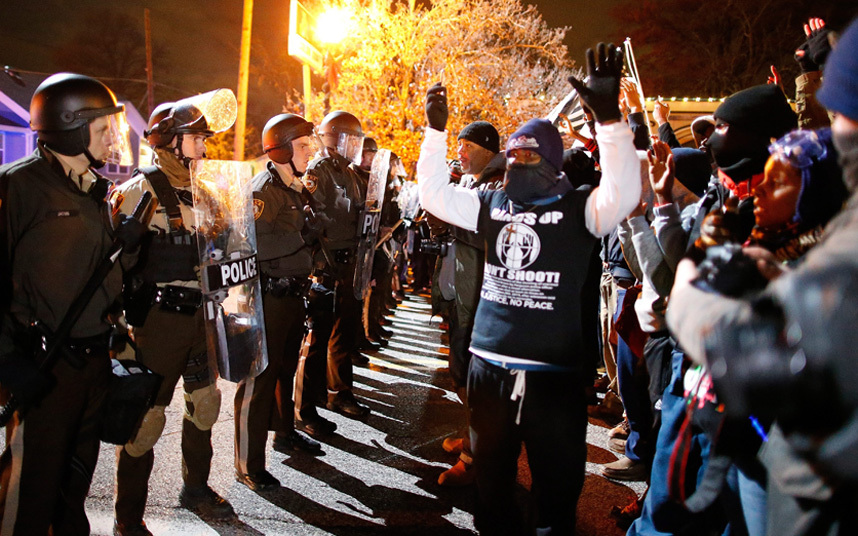
\includegraphics[width=8cm]{images/photos/ferguson_riots.jpg}
\caption{Photo of the Ferguson riots. On the left, policemen, on the right, protesters raising hands and saying "Don't Shoot"}
\end{wrapfigure}

On the August 9, 2014, a 18-year-old black man called Michael Brown is shot dead in Ferguson by a white police officer. This event was the trigger of riots, both peaceful and violent, for more than 2 weeks. 

As for former unrests, the Ferguson protest has been widely broadcasted on socials medias like Twitter. 

Lorem\\
Lorem\\
Lorem\\Lorem\\
Lorem\\
Lorem\\
Lorem\\

Some people, like Antonio French, were particularly active. Although not being a journalist, but leaving near Ferguson, he reported daily through Twitter what was happening in the field.

\begin{figure}[H]
\begin{minipage}[t]{0.48\textwidth}
\begin{center}
	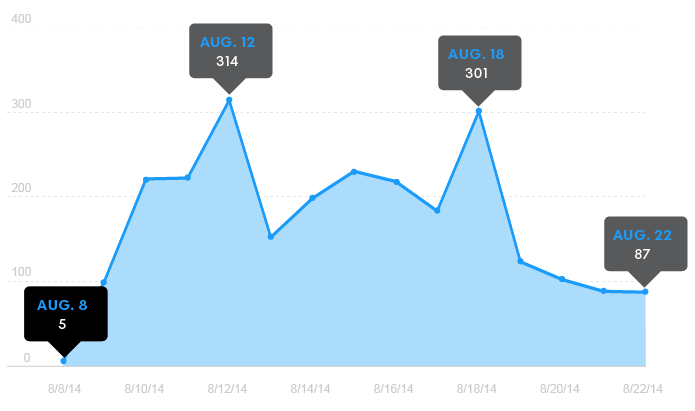
\includegraphics[width=\textwidth]{images/freqs/intro/af_tweets.png}
	\caption{A. French's tweets counts per day (\copyright \texttt{ usatoday.com})}
	\label{af_tweets}
\end{center}
\end{minipage}
\hfill
\begin{minipage}[t]{0.48\textwidth}
\begin{center}
	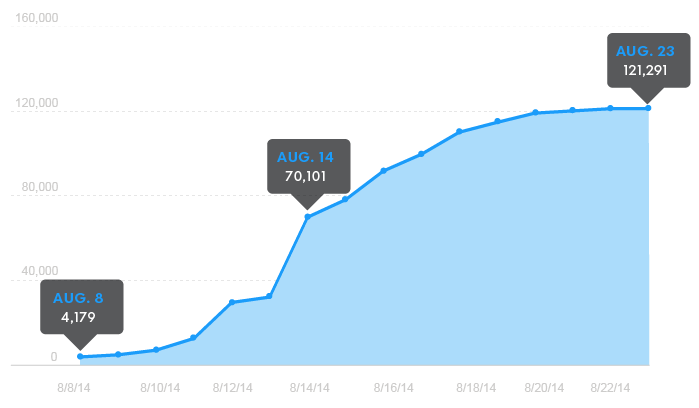
\includegraphics[width=\textwidth]{images/freqs/intro/af_followers.png}
	\caption{A. French's followers count evolution (\copyright \texttt{ usatoday.com})}
	\label{af_followers}
\end{center}
\end{minipage}
\end{figure}

In an article\footnote{http://www.usatoday.com/story/news/nation-now/2014/08/25/antonio-french-twitter-ferguson/14457633/} from USA Today, one can see on the figure \ref{af_tweets} how Antonio French was active (up to 300 tweets a day) during the whole unrest. And, even more interesting, the figure \ref{af_followers} shows how he became popular, as he was followed by more than 120,000 people, whereas he was almost unknown on Twitter before the protest. 

As the articles shows through examples tweets, Antonio French was in an informative role. He mostly posted pictures and videos during each riots, and tried everytime to gather information about what was happening. 

In this way, it is interesting to wonder how to model such a \emph{role} on Twitter during a riot and how to group users giving the \emph{role} they play.

\newpage

\section{Problem definition and objectives}

In this part we define the problem and we introduce clearly the objectives.

\begin{defbox}
\textbf{Definition} - Protest $\mathcal{P}_n$\\
A protest $\mathcal{P}_n$ is defined as a time ordered list of $n$ riots $r$.
$$ \mathcal{P}_n = [r_1, r_2, \cdots, r_n]$$
In our case, we suppose there is a riot each night. As a consequence, $\mathcal{P}_n$ is $n$-days long.
\end{defbox}

\begin{defbox}
\textbf{Definition} - Riot $r$ and topics $t$\\
A riot $r$ is defined as a set of $m$ topics $t$ occuring during the riot $r$.
$$ r = [t_1, t_2, \cdots, t_n]$$
A topic is itself a set of tweets, such as a tweet can belongs to several topics.
\end{defbox}



\begin{objbox}\color{Maroon}
\textbf{Objective 1 - Polarity} : define and compute the polarity of a user.
\end{objbox}

\begin{objbox}\color{Maroon}
\textbf{Objective 2 - Influence} : define and compute the influence of a user.
\end{objbox}

\begin{objbox}\color{Maroon}
\textbf{Objective - Role} : define and compute the role of a user, and then the distance and similarity between two users.
\end{objbox}

\newpage
\section{Outline}

\newpage

\section{Organisation and methods}

This project has been conducted between February and May...


%%%%%%%%%%%%%%%%%%%%%%%%%%%%%%%%%%%%%%%%%%%%%%%%%%%%%%%%%%%%%%%%%%%%%%%
%%%%%%%%%%%%%%%%%%%%%%%%%%%%%%%%%%%%%%%%%%%%%%%%%%%%%%%%%%%%%%%%%%%%%%%
%%%%%% CHAPTER 2 - DATASET
%%%%%%%%%%%%%%%%%%%%%%%%%%%%%%%%%%%%%%%%%%%%%%%%%%%%%%%%%%%%%%%%%%%%%%%
%%%%%%%%%%%%%%%%%%%%%%%%%%%%%%%%%%%%%%%%%%%%%%%%%%%%%%%%%%%%%%%%%%%%%%%

\chapter{Dataset (10p)}

\section{Origin}
Obtaining datasets about riots is not a simple task. Twitter does not allow to fetch past tweets between two dates with a precise keyword, but only new tweets from the Stream API. Some research groups manage to grant a special access from Twitter, like for the London riots study[REF], but do not make these datasets publicly available online.

Moreover, Twitter does not allow neither peers to share full datasets obtained with its API. However, the company allows people for now to share IDs list of tweets, without any content. One is then able to use the Twitter API to fetch, for each ID, the tweet content (text, author, date etc.) under the rates limitations.

The dataset used in this project is obtained from Ed Summers, a developer who started to record the Ferguson-related tweets after Mike Brown's shooting and who published on his blog the IDs list\footnote{\url{http://inkdroid.org/journal/2014/08/30/a-ferguson-twitter-archive/}}.

The task was then to \emph{hydrate} the tweets and users to obtain the full dataset.

\newpage

\section{Structure}
The dataset contains approximately 12 million tweets and contains data from the 10 August to the 27 August.

\subsection{Tweet structure}
plop
\begin{figure}[h!]
\centering
\begin{tabular}{c|c|c}
field & type & example\\
\midrule
id & number & \texttt{498619822134280192} \\ \hline
publication date & date & \texttt{2014-08-11 00:00:04} \\ \hline
author id & number & \texttt{124010717} \\ \hline
text & number & \pbox{9cm}{\vspace*{5pt}\texttt{Please follow @AntonioFrench now! \newline \#Ferguson \#MikeBrown http://t.co/---}\vspace*{5pt}} \\ \hline
retweet count & number & \texttt{4} \\ \hline
is it a retweet ? & boolean & \texttt{False} \\ \hline
hashtags & string list & \texttt{\#Ferguson, \#MikeBrown} \\ \hline
links and medias & string list & \texttt{http://t.co/---} \\ \hline
\end{tabular}
\caption{Tweet schema}
\end{figure}

\subsection{User structure}
plop
\begin{figure}[h!]
\centering
\begin{tabular}{c|c|c}
field & type & example\\
\midrule
user id & number & \texttt{14090948} \\ \hline
name & string & \texttt{Antonio French} \\ \hline
nickname & string & \texttt{AntonioFrench} \\ \hline
registration date & date & \texttt{2008-03-06 19:51:29} \\ \hline
tweet count & number & \texttt{19372} \\ \hline
followers count & number & \texttt{119977} \\ \hline
friends count & number & \texttt{1373} \\ \hline
\end{tabular}
\caption{User schema}
\end{figure}
Lorem\\
Lorem\\
Lorem\\
Lorem\\
Lorem\\
\newpage
\section{Basic analysis}

\subsection{Frequencies}

\begin{figure}[H]
\begin{minipage}[t]{0.48\textwidth}
\begin{center}
	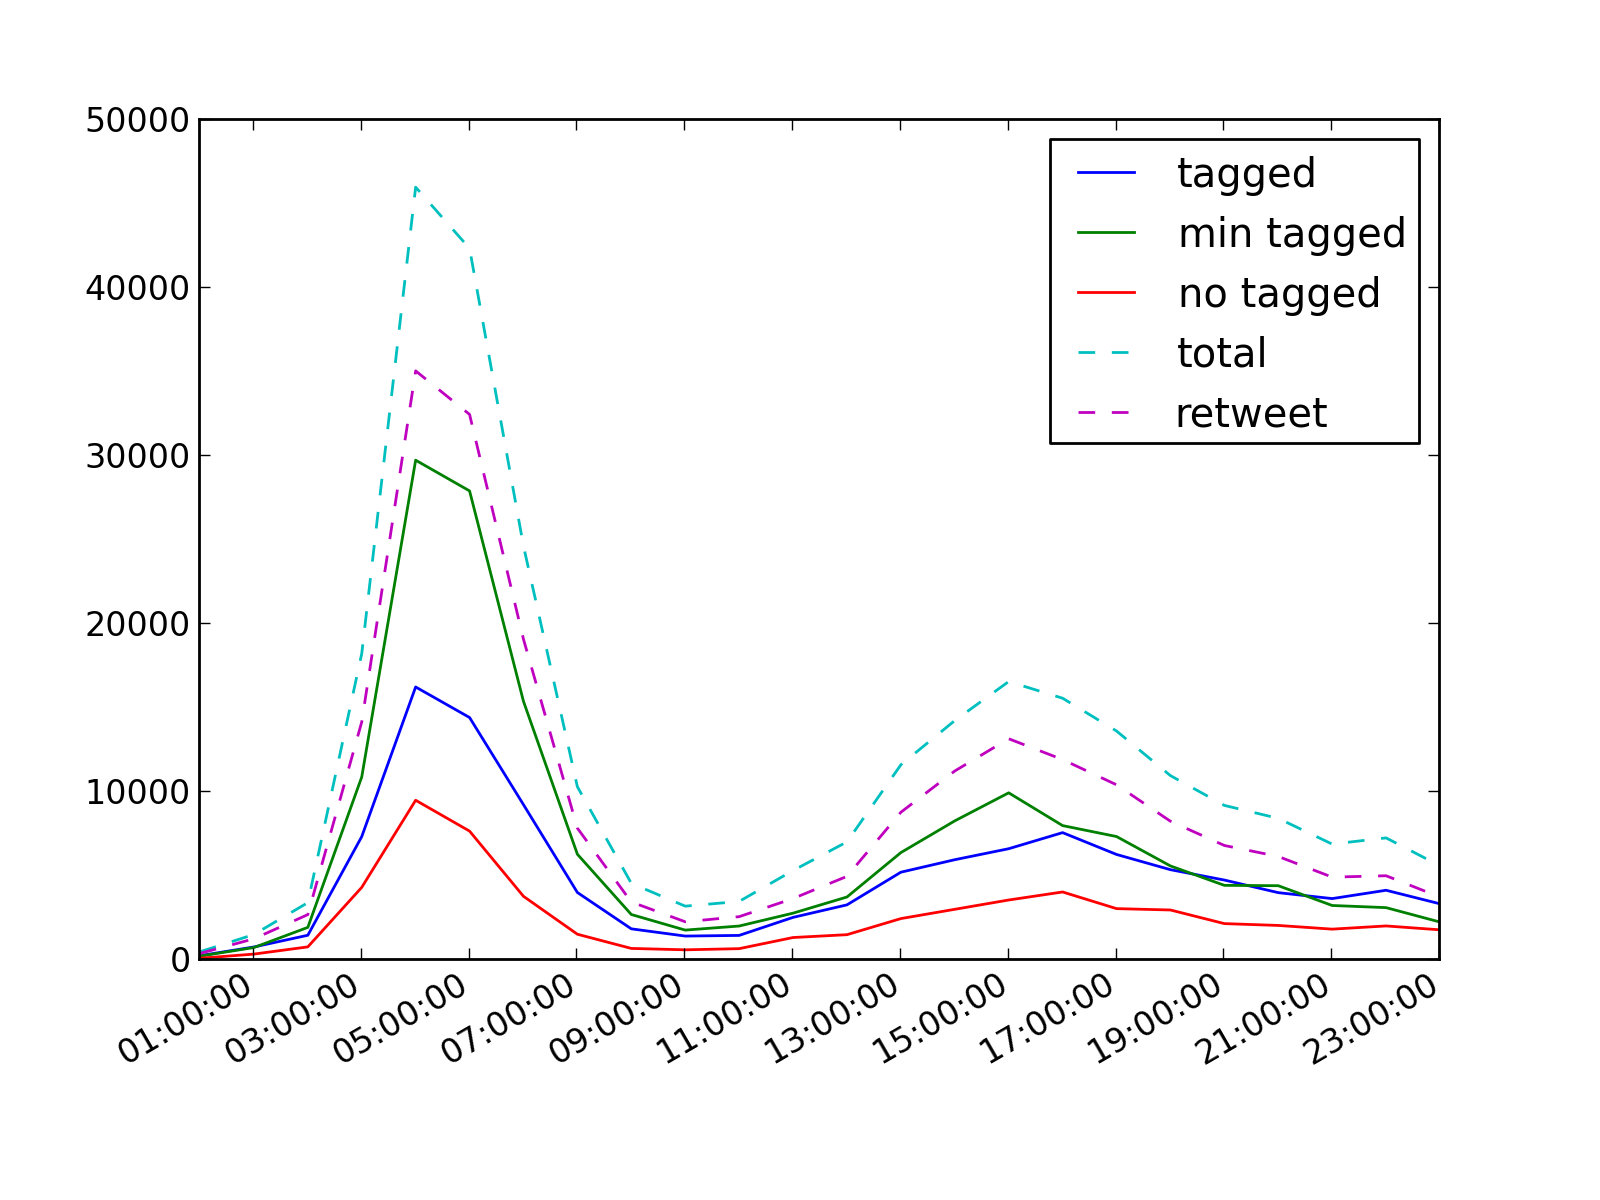
\includegraphics[width=\textwidth]{images/freqs/freq_11_08.png}
	\caption{11/08 : tweets frequencies}
\end{center}
\end{minipage}
\hfill
\begin{minipage}[t]{0.48\textwidth}
\begin{center}
	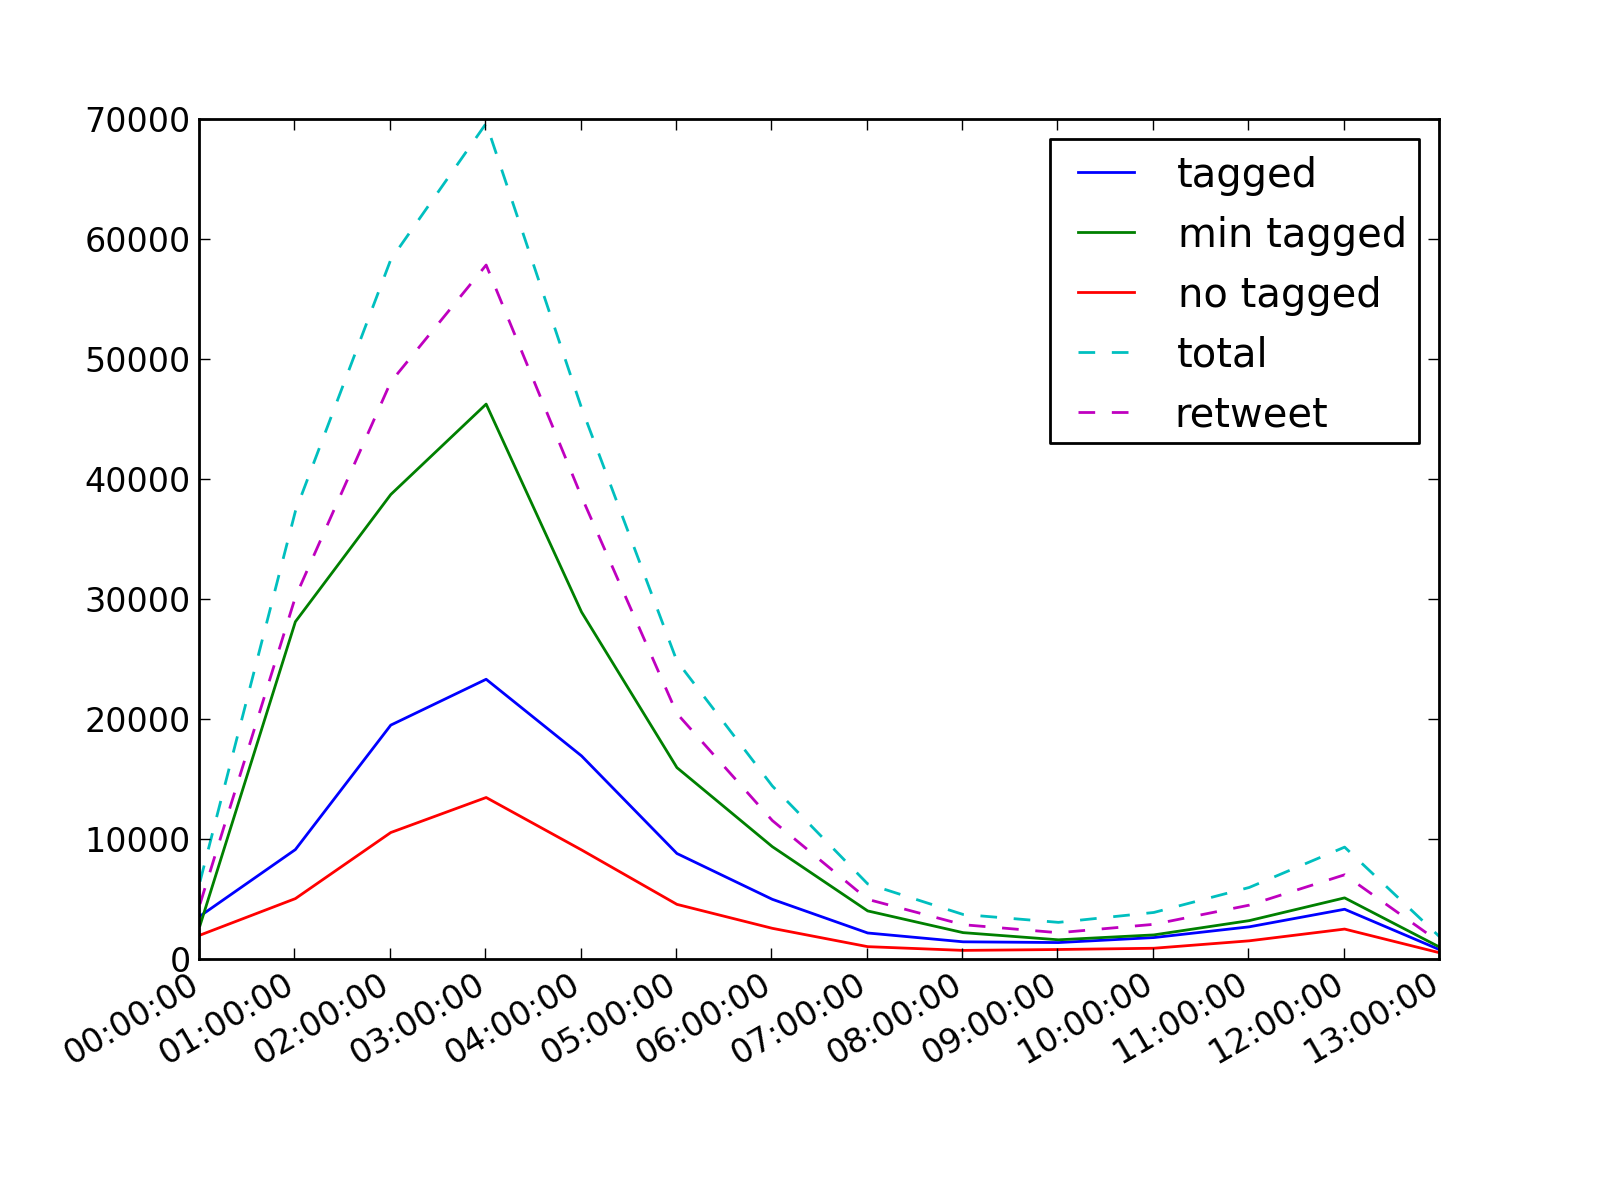
\includegraphics[width=\textwidth]{images/freqs/freq_12_08.png}
	\caption{12/08 : tweets frequencies}
\end{center}
\end{minipage}
\end{figure}

\begin{figure}[H]
\begin{minipage}[t]{0.48\textwidth}
\begin{center}
	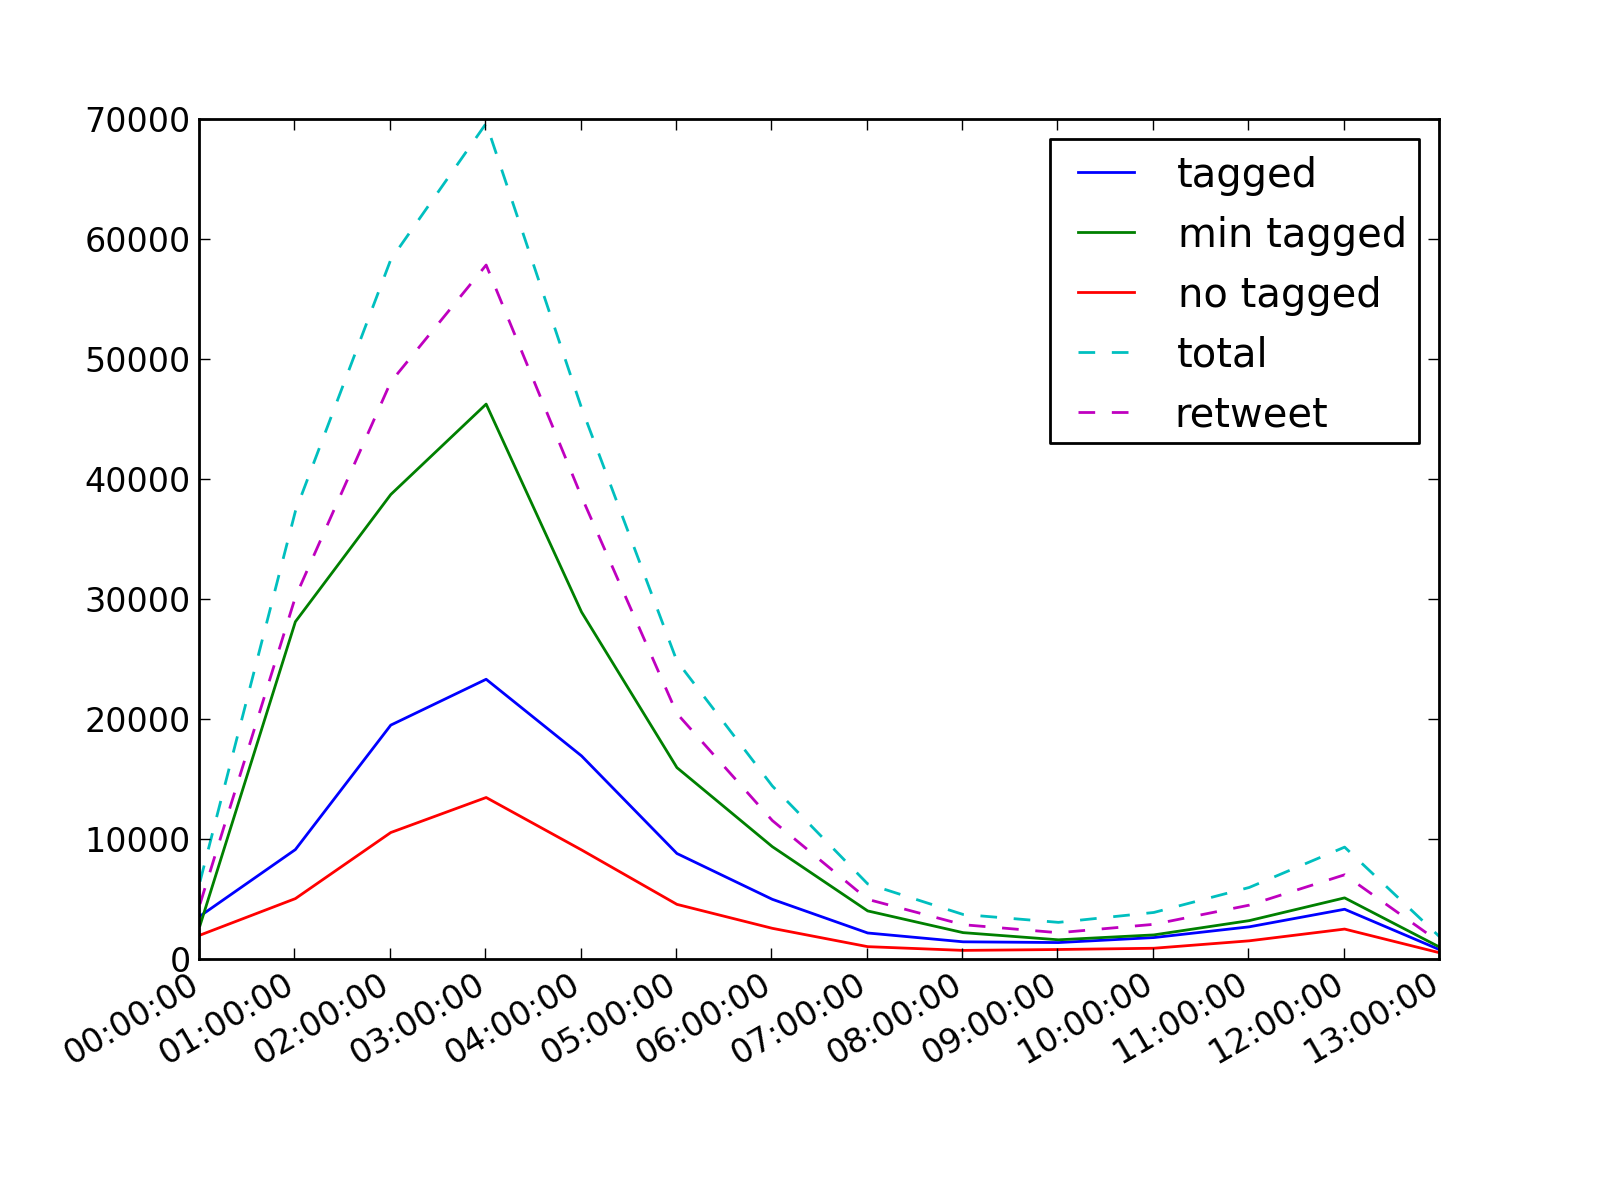
\includegraphics[width=\textwidth]{images/freqs/freq_12_08.png}
	\caption{13/08 : tweets frequencies}
\end{center}
\end{minipage}
\hfill
\begin{minipage}[t]{0.48\textwidth}
\begin{center}
	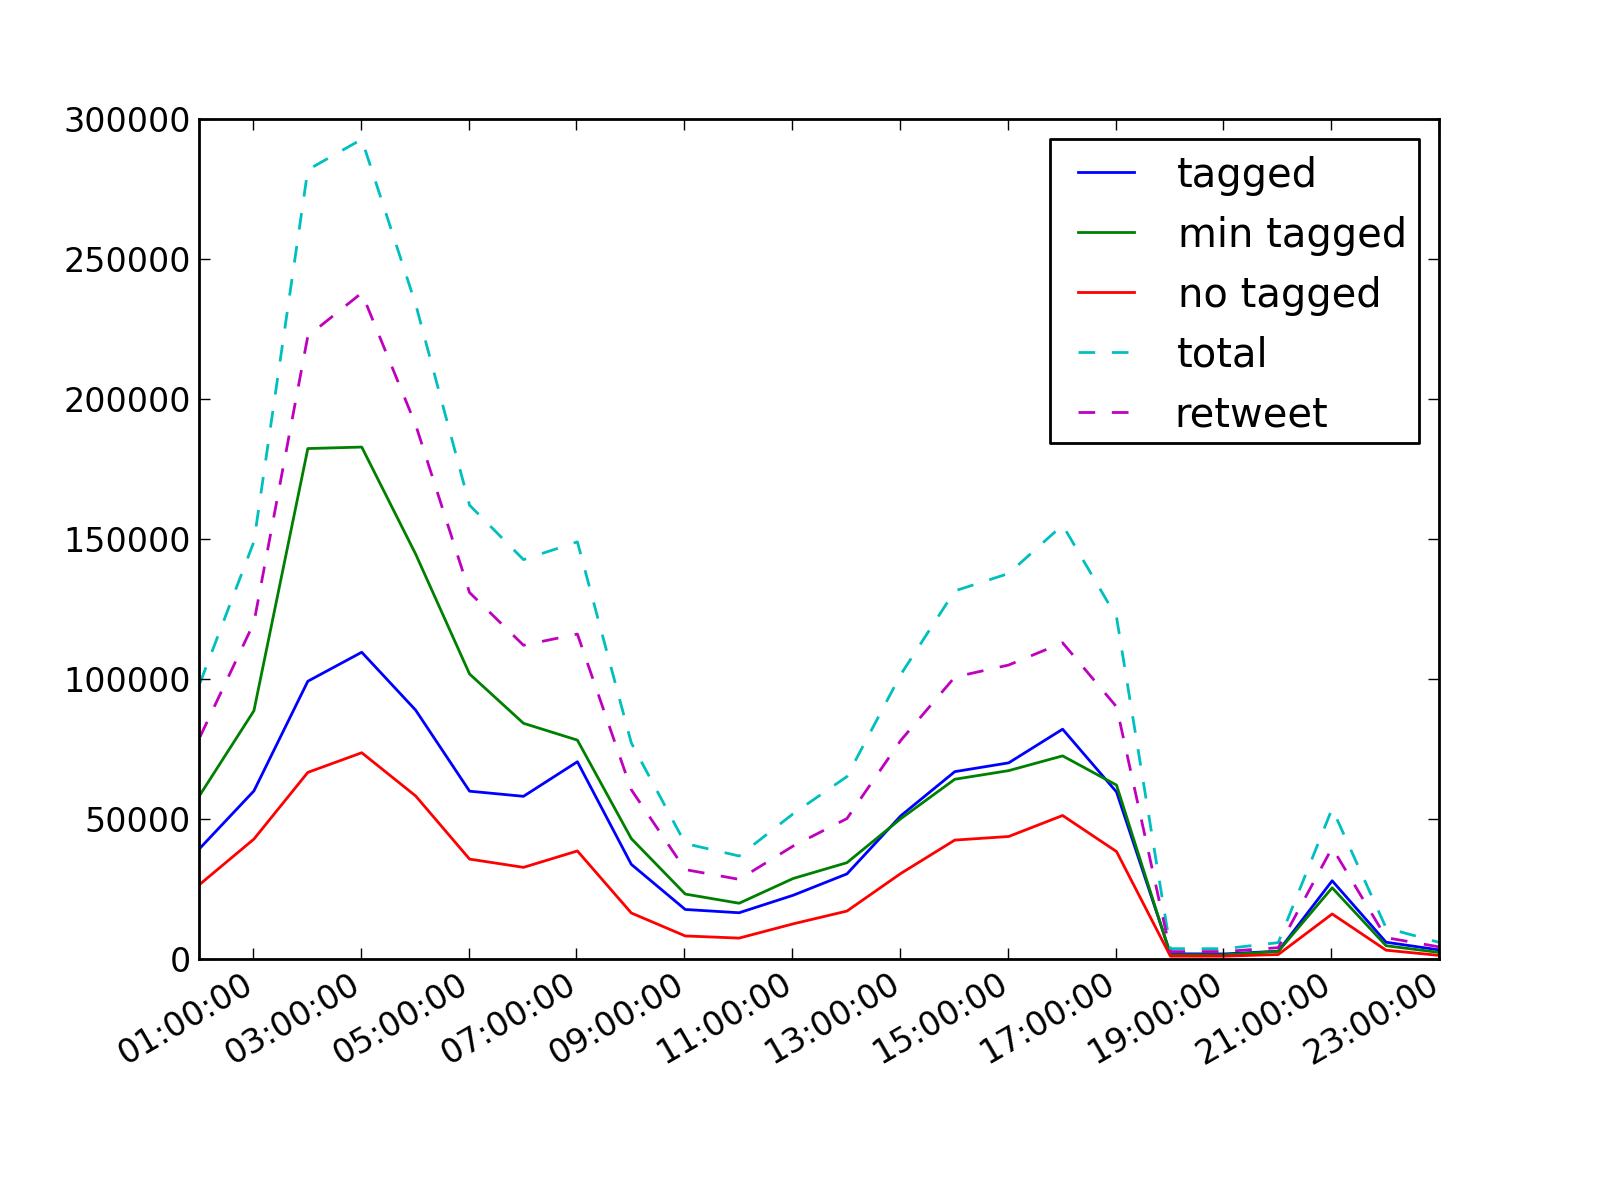
\includegraphics[width=\textwidth]{images/freqs/freq_14_08.png}
	\caption{14/08 : tweets frequencies}
\end{center}
\end{minipage}
\end{figure}

\begin{figure}[H]
\begin{minipage}[t]{0.48\textwidth}
\begin{center}
	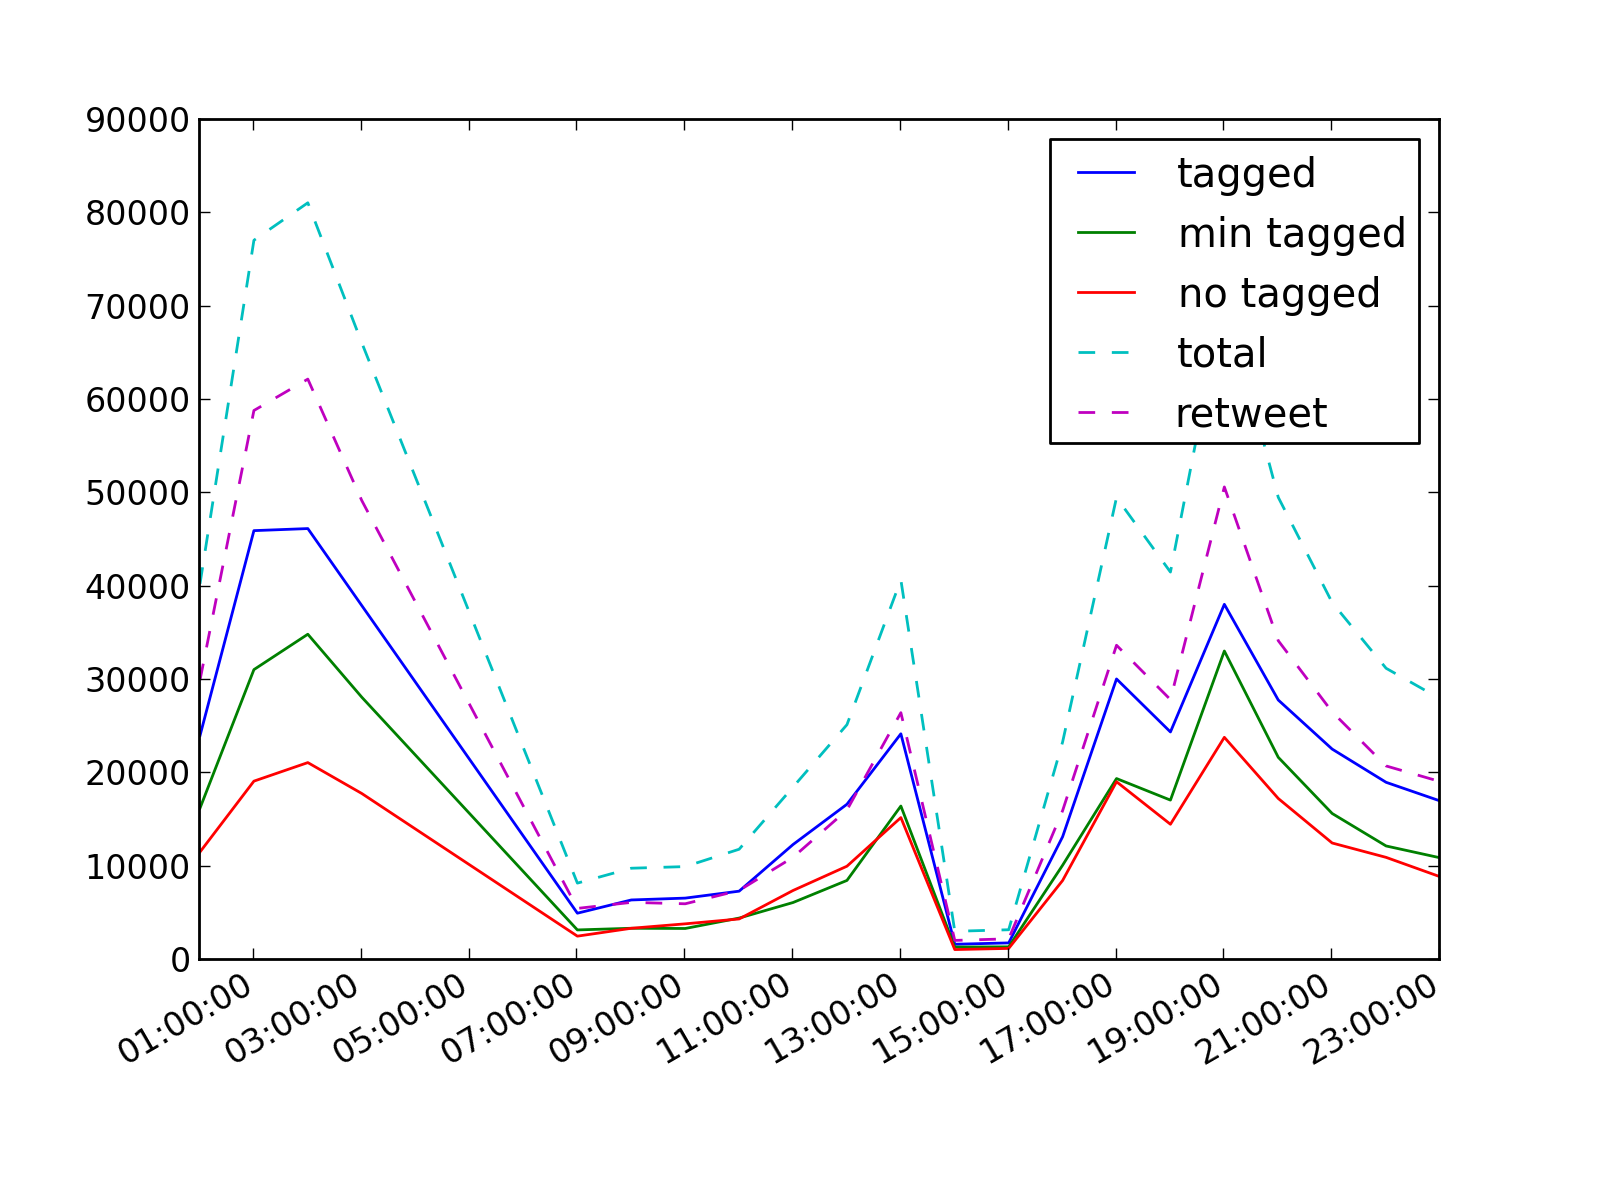
\includegraphics[width=\textwidth]{images/freqs/freq_15_08.png}
	\caption{15/08 : tweets frequencies}
\end{center}
\end{minipage}
\hfill
\begin{minipage}[t]{0.48\textwidth}
\begin{center}
	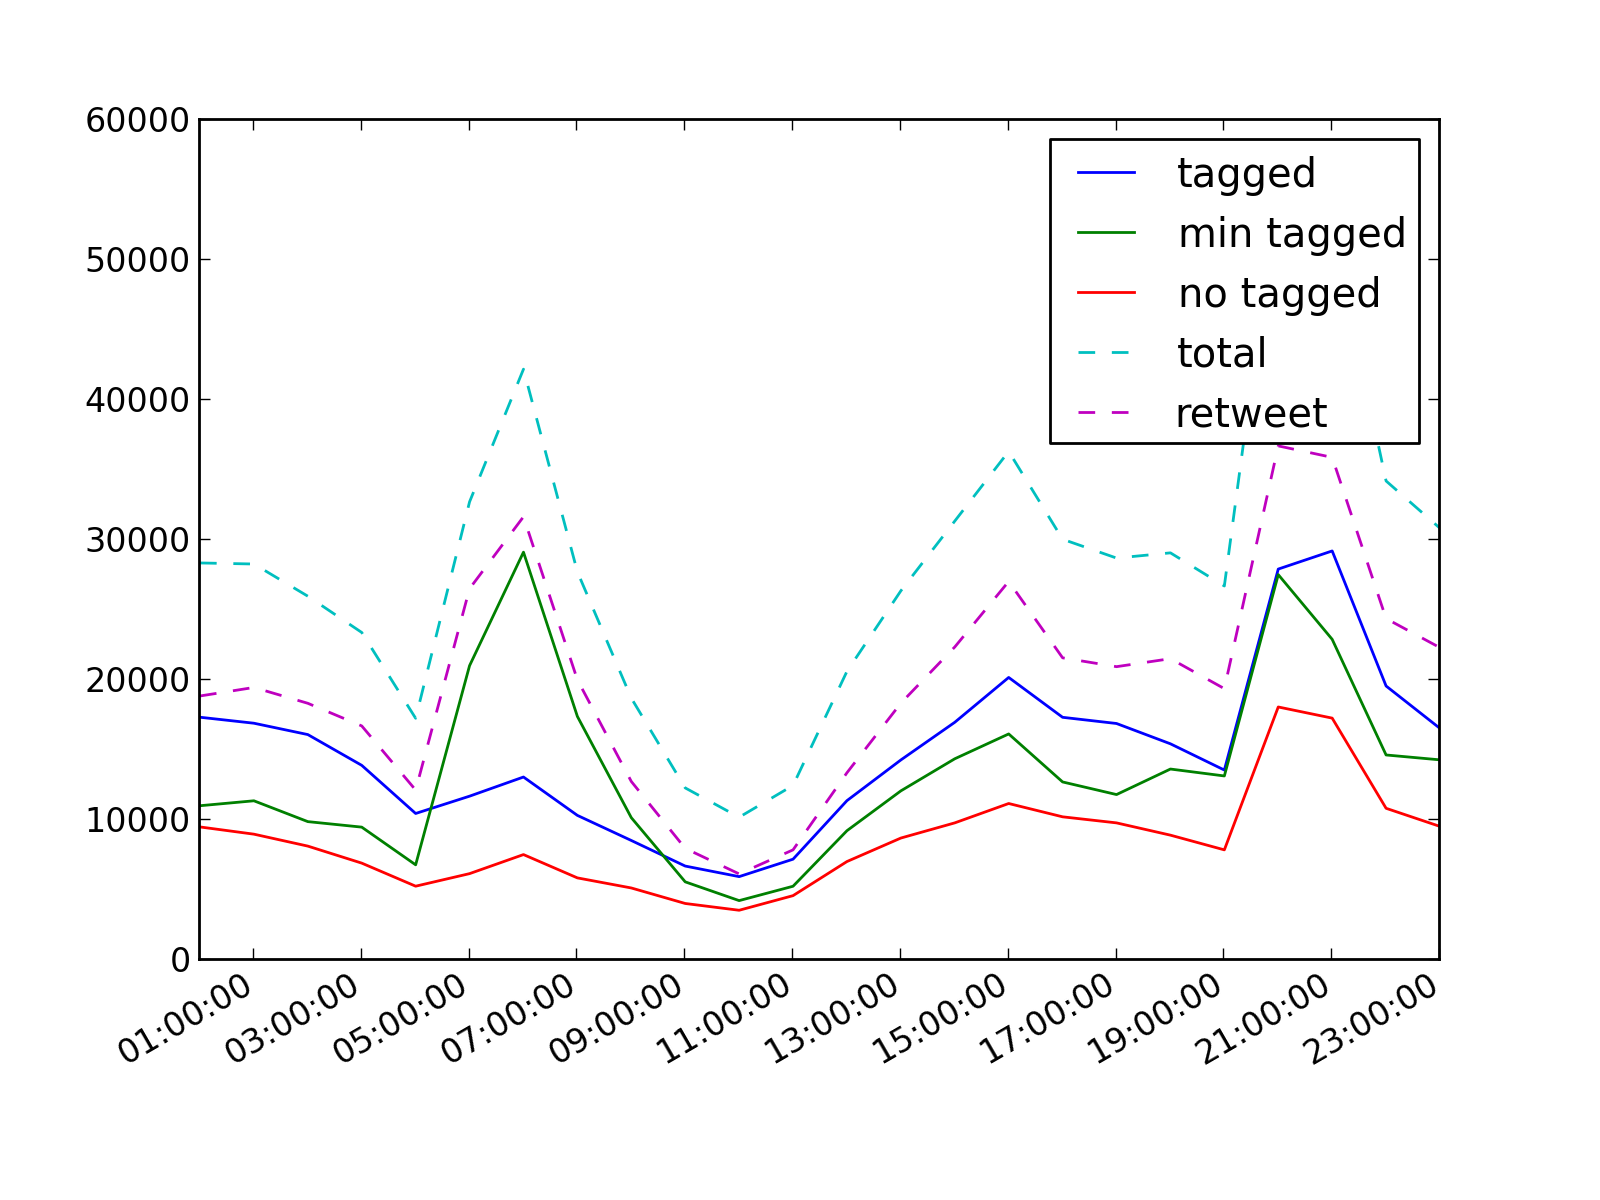
\includegraphics[width=\textwidth]{images/freqs/freq_16_08.png}
	\caption{16/08 : tweets frequencies}
\end{center}
\end{minipage}
\end{figure}

\newpage

%\subsubsection*{0am-2am (2,058 tweets)}
%\toprt{top_rt_11_08_00_02}
%\subsubsection*{2am-4am (22,297 tweets)}
%\toprt{top_rt_11_08_02_04}
%\subsubsection*{4am-7am (113,264 tweets)}
%\toprt{top_rt_11_08_04_07}

%%%%%%%%%%%%%%%%%%%%%%%%%%%%%%%%%%%%%%%%%%%%%%%%%%%%%%%%%%%%%%%%%%%%%%%
%%%%%%%%%%%%%%%%%%%%%%%%%%%%%%%%%%%%%%%%%%%%%%%%%%%%%%%%%%%%%%%%%%%%%%%
%%%%%% CHAPTER 3 - CONTENT POLARITY
%%%%%%%%%%%%%%%%%%%%%%%%%%%%%%%%%%%%%%%%%%%%%%%%%%%%%%%%%%%%%%%%%%%%%%%
%%%%%%%%%%%%%%%%%%%%%%%%%%%%%%%%%%%%%%%%%%%%%%%%%%%%%%%%%%%%%%%%%%%%%%%

\chapter{Language analysis and content polarity}
\section{Motivation}
In order to characterize the role of a user in a riot, the most straightfoward approach is to study what he says. A tweet allows a user to publish a 140 characters message. 

\section{Preprocessing}
Before analyzing the data, it's essential to preprocess it. 

\fbox{
  \parbox{\textwidth}{\texttt{
\colorbox{red!20}{RT @kharyp:} How police treat white opencarry supporter vs an unarmed black teen. Wonder why? \colorbox{red!20}{\#MikeBrown} \colorbox{red!20}{\#Ferguson} \colorbox{red!20}{http://t.co/jG3hGJRAuC}
}
  }
}

\begin{enumerate}
\item \textbf{\underline{Cleaning} :} we remove all the non textual items : 
  \begin{itemize}
    \item mentions
    \item hashtags
    \item urls
  \end{itemize}
\fbox{
  \parbox{0.9\textwidth}{\texttt{
How police treat white opencarry supporter vs an unarmed black teen. Wonder why?}
  }
}
\item \textbf{\underline{Tokenization} :} breaks the sentence into a list of tokens, that can be words or symbols (punctuation). The tokens order is not considered anymore and a token can appear several time in the list.  \\[10pt]
\fbox{
  \parbox{0.9\textwidth}{\texttt{
how, police, treat, white, opencarry, supporter, vs, an, unarmed, black, teen, ., wonder, why, ?}
  }
}
\item \textbf{\underline{Punctuation and Stop words removing} :}  keeps only the valuable tokens by removing symbols and too common words like \emph{what}, \emph{and}, \emph{of} etc.\\[10pt]
\fbox{
  \parbox{0.9\textwidth}{\texttt{
police, treat, white, opencarry, supporter, vs, unarmed, black, teen, wonder}
  }
}
\item \textbf{\underline{Stemming} :} keeps the stem of words, such as for example \emph{unarmed} and \emph{unarm} will be the same token. This process reduces the vocabulary and allows to compare more easily token lists.\\[10pt]
\fbox{
  \parbox{0.9\textwidth}{\texttt{
police, treat, white, opencarry, supporter, vs, unarm\st{ed}, black, teen, wonder}
  }
}

\end{enumerate}

\section{Supervised classification : characterizing tweets by type}
Supervised learning is helpful because one can choose the categories. 

Concerning a riot, a useful approach is to classify tweets by their types. We establish a simple type classification below.

\subsection{Intuition}

\newcommand{\info}[1]{\colorbox{cyan!20}{#1}}
\newcommand{\rass}[1]{\colorbox{red!20}{#1}}
\newcommand{\ninfo}[1]{\colorbox{black!20}{#1}}
\newcommand{\nrass}[1]{\colorbox{green!20}{#1}}

By taking a look at some tweets obtained on the 11th of August, we can underline several types of tweets and construct the following classification :

\begin{figure}[h!]
\centering
\begin{tabular}{l|m{7cm}|m{6cm}}
type & details & example\\
\hline
\hline
\info{informative} & The tweet contains informative text content about the happening riot. The URL link is ignored. & "\#Ferguson quiktrip burning http://t.co/1Jm5ngZe62" \\
\hline
\ninfo{non informative} & The tweet expresses feeling, an idea, a conviction, but no information about the happening riot. & "Prayers for \#STL \#Ferguson." \\
\hline
\hline
\rass{involved} & The tweet support, encourages directly the happening riot, the rioters or their ideas. & "Just spread the word we need \#Justice" \#ferguson \#stlouis \#MO  \#uniteblue \#libcrib \#p2 http://t.co/78QURveWvK" \\
\hline
\nrass{not involved} & The tweet is objective about the situation or blame the riot, the riotes or their ideas. & "I am beyond saddened to see the looting in \#Ferguson. This removes the focus from justice for \#MikeBrown. Violence is never an answer." \\
\end{tabular}
\end{figure}

The figure \ref{tabtypes} shows more example of manually classified tweets. The second column highlights semantical or syntaxical details that helps to classify the given tweet.
One can notice the types pairs appearing, mostly :

\begin{itemize}
\item \info{informative}/\nrass{not involved} : tweets of interest as they are describing the riot situation in an objective way, for example eyewitnesses.
\item \ninfo{non informative}/\rass{involved} : useful tweets as their authors support the riot. It's interesting to consider the content in order to :
\begin{itemize}
\item understand the rioters claims ;
\item observe if the "virtual violence" (language for example) of these users evolves ;
\item identify the main influencers.
\end{itemize}
\end{itemize}

The two others types are less interesting. Indeed, \ninfo{non informative}/\nrass{not involved} tweets does not contain any valuable information and \info{informative}/\rass{involved} tweets should be avoided as they may not contain objective information.

\begin{figure}[h!]
\centering
\begin{tabular}{c|Cp{3cm}}
id & content & type \nl
1 & "A riot is the language of the unheard." $~$Martin Luther King, Jr. \#Ferguson http://t.co/OXfzgEcN1B & \ninfo{non informative} \newline \nrass{not involved} \nl
2 & The Watts Riots began on \info{August 11, 1965}.  \info{49} years ago today. \#Ferguson http://t.co/gYgaI5WlP9 & \info{informative} \newline \nrass{not involved} \nl
3 & QuickTrip is \info{burning} to the ground. \#Ferguson http://t.co/9ykNn4a8ek & \info{informative} \newline \nrass{not involved} \nl
4 & \ninfo{Prayers} for \#STL \#Ferguson. & \ninfo{non informative} \newline \nrass{not involved} \nl
5 & The QuickTrip is \info{now} \info{burning}. \#Ferguson (photo: @PDPJ) http://t.co/tJBeXQ6hzF & \info{informative} \newline \nrass{not involved} \nl
6 & "if you Retweet or Screenshot. Just \rass{spread the word} \rass{we need \#Justice}" \#ferguson \#stlouis \#MO  \#uniteblue \#libcrib \#p2 http://t.co/78QURveWvK & \ninfo{non informative} \newline \rass{involved}  \nl
7 & \info{Tear gas} is being used in \#Ferguson.  Mayor tells \info{CNN} he has been receiving death threats. \info{Armored vehicles roam the streets}. & \info{informative} \newline \nrass{not involved} \nl
8 & \rass{PAY ATTENTION} as "teen" becomes "man," "community" becomes "mob," and \rass{"murder" becomes "alleged shooting}." \#Ferguson \rass{\#medialiteracy} & \ninfo{non informative} \newline \rass{involved} \nl
9 & \info{Happening now} in \#Ferguson http://t.co/KFuaOEZ4tf & \info{informative} \newline \nrass{not involved} \nl
10 & \rass{Nothing has changed}. The ONLY difference?  The pictures are in color.  \#Ferguson \#FergusonShooting http://t.co/7p23qyDGwY & \ninfo{non informative} \newline \rass{involved} \nl
11 & \#Ferguson quiktrip \info{burning} http://t.co/1Jm5ngZe62 & \info{informative} \newline \nrass{not involved} \nl
12 & \info{Men} have \info{pulled} a \info{truck} up to the QT and are loading the ATM into the back. \#Ferguson & \info{informative} \newline \nrass{not involved} \nl
13 & \info{SWAT Team}. Taco Bell. \#Ferguson (photo:@kodacohen) http://t.co/Mo8CDVWx32 & \info{informative} \newline \nrass{not involved} \nl
14 & \info{Shots} \info{fired} at Walmart. \#Ferguson & \info{informative} \newline \nrass{not involved} \nl
15 & I am beyond saddened to \info{see the looting} in \#Ferguson. This removes the focus from justice for \#MikeBrown. \nrass{Violence is never an answer}. & \info{informative ?} \newline \nrass{not involved} \nl
\end{tabular}
\label{tabtypes}
\caption{Example of labelization}
\end{figure}

\newpage 

\begin{figure}[h]
\centering
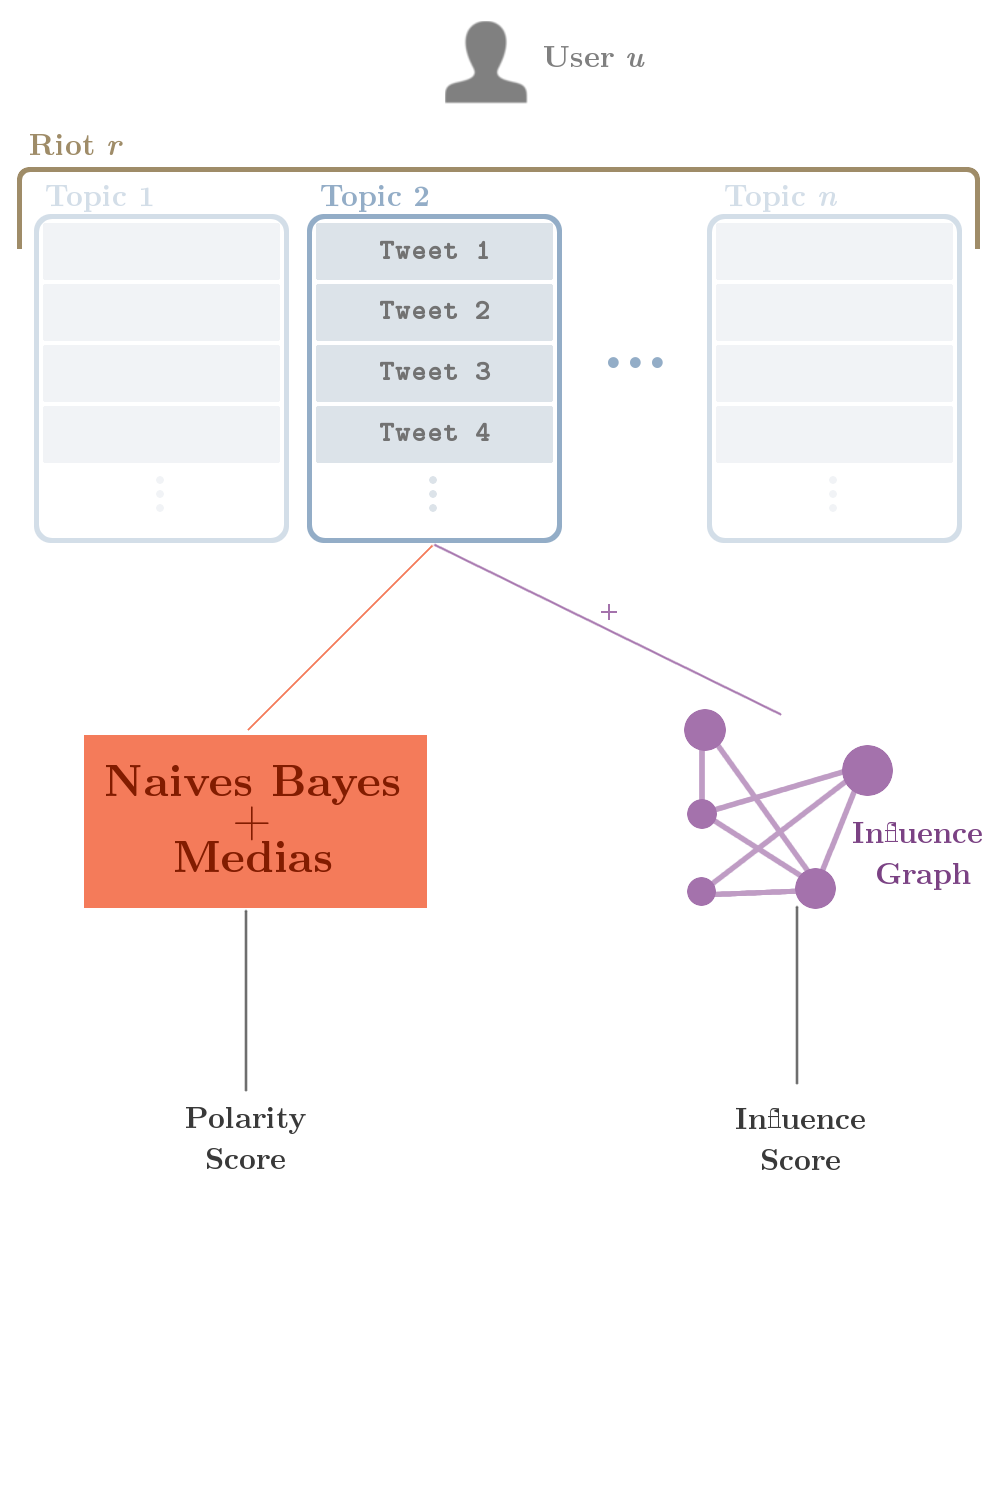
\includegraphics[width=0.8\textwidth]{images/diags/chain.png}
\caption{plop}
\end{figure}

\subsection{Multinomial Naives Bayes Classifier}

The model used is the Multinomial Naive Bayes, a well-used probabilistic learning method.
The Naive Bayes is a supervised method, which means its learns from a labelled dataset called training set. Once the model is trained, it can be used on unlabelled data. In order to measure the model accuracy, we run is on a test dataset.

\subsubsection{Naives Bayes}
Let $ \mathcal{D} = \{ d_i \}_{0\leq i\leq n} $ be the set of $n$ documents in the dataset.

For each document $d_i$, let $x_{1},x_{2},\cdots,x_{m}$ be its $m$ features, such as $$d_i = (x_{1},x_{2},\cdots,x_{m})$$
Let's assume the features are independent.

The probability that the document $d_i$ belongs to class $C_k$ is given by :
$$ P(C_k|d_i) = \frac{P(C_k)P(d_i|C_k)}{P(d_i)} $$
i.e. $$ P(C_k|x_{1},\cdots,x_{m}) = \frac{P(C_k)\prod_{j=1}^mP(x_{j}|C_k)}{P(d_i)} $$

The predicted class $\hat{C}$ is then given by the class that has the maximum probability :

$$ \hat{C} = \arg \max_k P(C_k|x_{1},\cdots,x_{m}) $$

\subsubsection{Word representation}

In our case, a document can be represented as a bag of words, which is a set where the word frequency is considered.

For example, given a document $d$ : \fbox{\texttt{prayers,mike,brown,prayers,ferguson}}

A bag-of-words representation would be :
\begin{center}
\begin{tabular}{|c|c|c|c|}
prayers & mike & brown & ferguson \\
2 & 1 & 1 & 1
\end{tabular}
\end{center}

Considering several documents as a dataset, we define the vocabulary $\mathcal{V}$ as the set of all the words existing in the dataset.

Continuing on the previous example, if $\mathcal{V}$ is defined as $\{\textsf{brown, ferguson, fire, mike, police, prayers, riots}\}$, the document $d$ can be represented as a count vector :

$$
\bordermatrix{~ & brown & ferguson & fire & mike & police & prayers & riots \cr d =  & 1 & 1 & 0 & 1 & 0 & 2 & 0 \cr}
$$

This is a multinomial document representation.

\subsubsection{Multinomial Naives Bayes}
The Multinomial Naives Bayes is a common variant for text classification.

$$ 
\boxed{P(x_{j}| C_k ) = \frac{N_{k,j} + \alpha}{N_k + \alpha n}}
$$

with 
\begin{itemize}
\item $N_{k,j}$ the count of the feature $x_j$ in the class $C_k$
\item $N_{k}$ the total count for all the features in $C_k$
\item $\alpha$ is a smoothing parameter, such that $\alpha \leq 1$, to avoid a zero value in the product of the naives bayes equation.
\end{itemize}


\subsubsection{Training the model}
In order to train our model, we manually label 500 tweets randomly choosen from the first riot (11 August). We annotate each document with two labels as follow : 

\begin{center}
\begin{tabular}{ccc}
informativness & involvement & ~ \\ \hline
0 & 0 & $\neg$ informative \& $\neg$ involved \\ \hline
0 & 1 & $\neg$ informative \& involved \\ \hline
1 & 0 & informative \& $\neg$ involved \\ \hline
1 & 1 & informative \& involved \\ \hline
\end{tabular}
\end{center}

\begin{figure}[H]
\centering
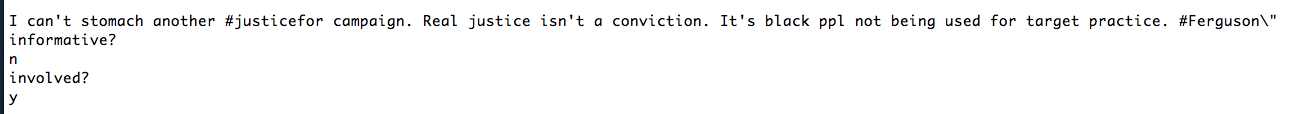
\includegraphics[width=\textwidth]{images/screens/manual_label_screen.png}
\caption{plop}
\end{figure}

\newpage

\begin{multicols}{2}[\textbf{Tweet type repartition on a manually classified 500 tweets sample}]

\begin{figure}[H]
\centering
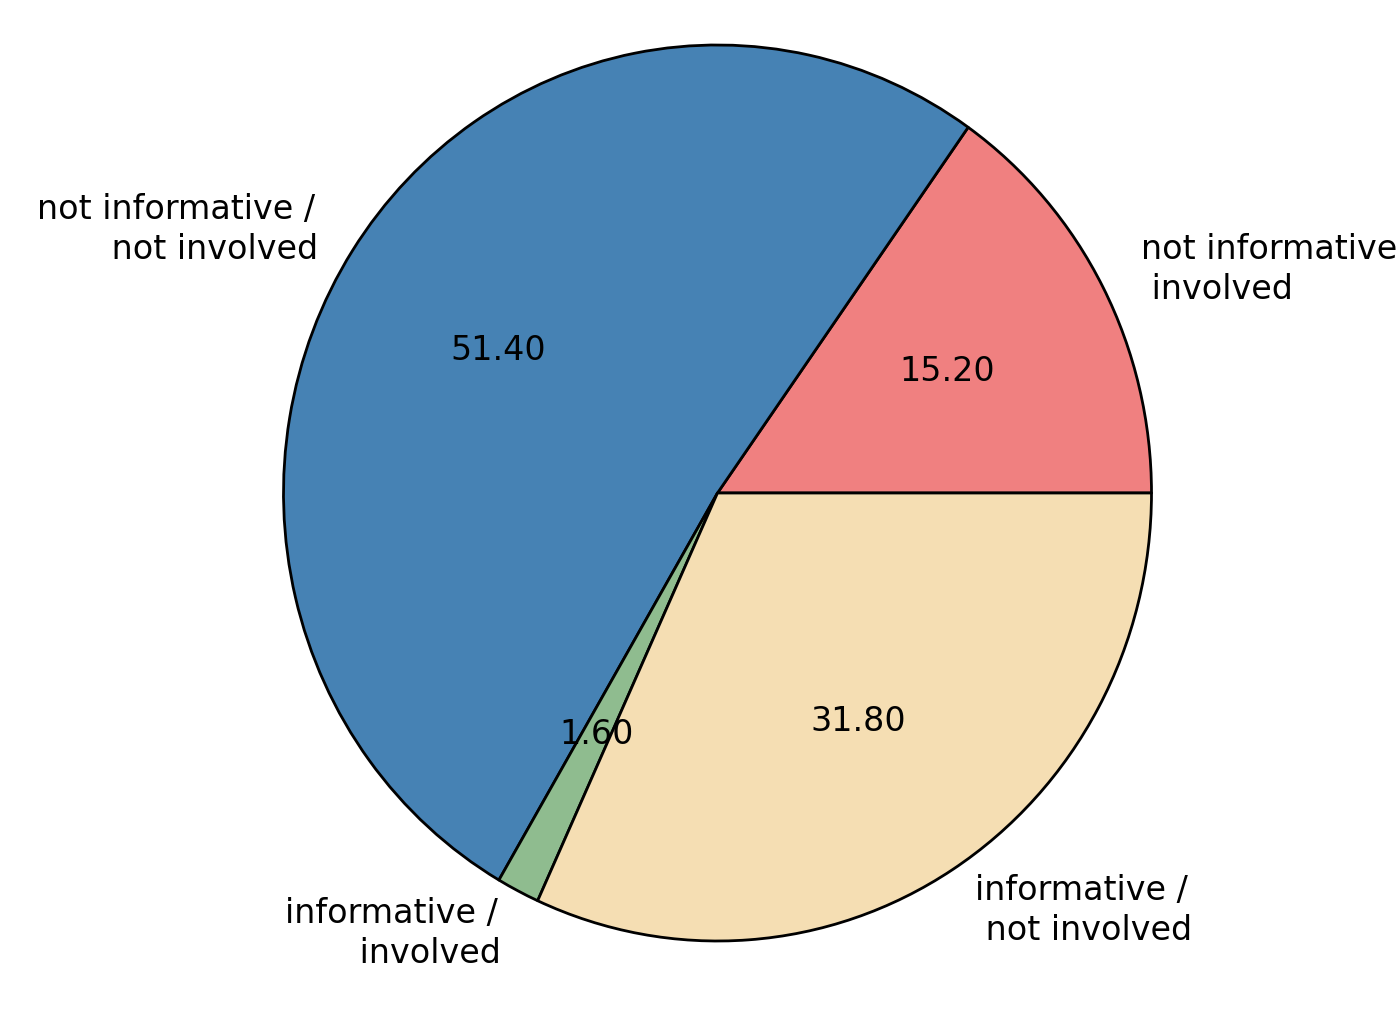
\includegraphics[width=0.5\textwidth]{images/plots/pies/pie_pairs.png}
\caption{Tweets type repartition for the informative and involved features}
\label{pieTypeInfInv}
\end{figure}
\begin{figure}[H]
\centering
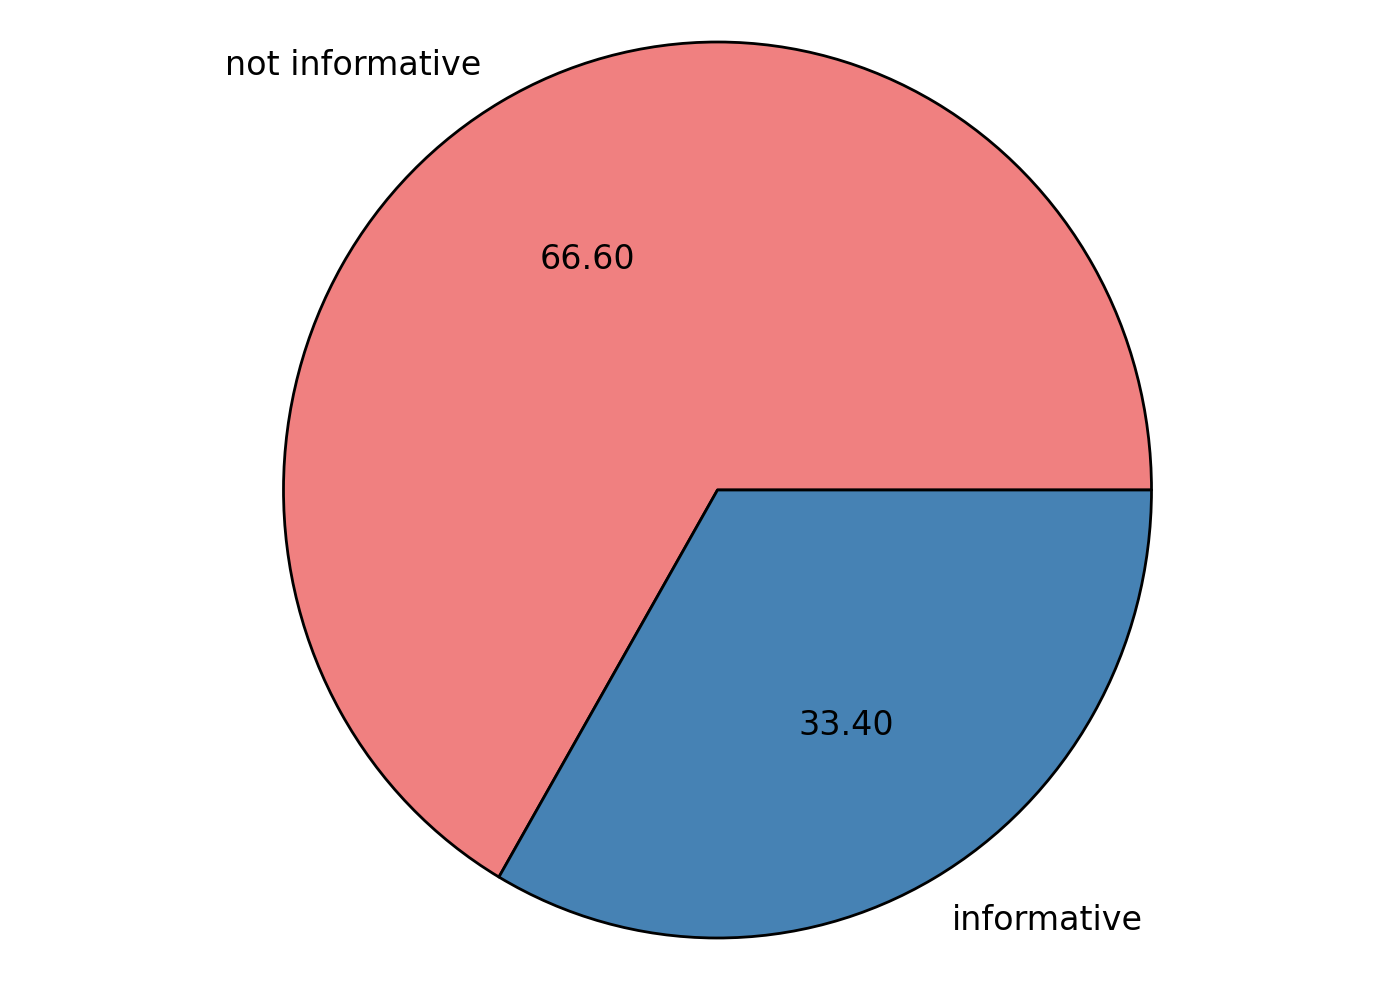
\includegraphics[width=0.5\textwidth]{images/plots/pies/pie_info.png}
\caption{Tweets type repartition for the informative feature}
\label{pieTypeInf}
\end{figure}
\begin{figure}[H]
\centering
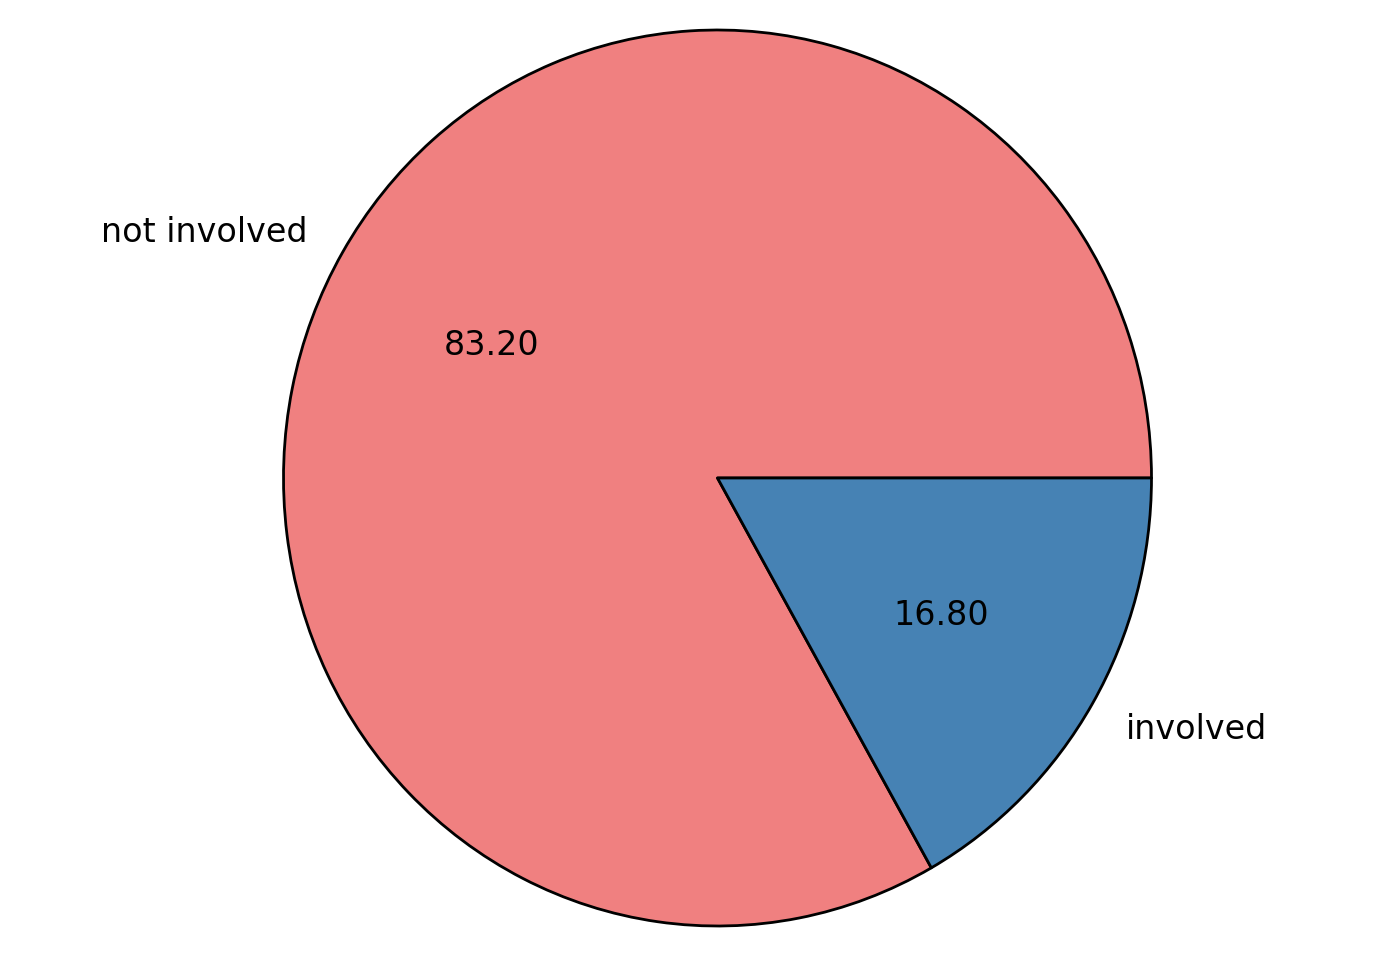
\includegraphics[width=0.5\textwidth]{images/plots/pies/pie_invo.png}
\caption{Tweets type repartition for the involvement feature}
\label{pieTypeInv}
\end{figure}
\vfill
To visualize the repartition of the features informative and involvement, we plot the following pies.\\
Firstly, one can notice on the figure \ref{pieTypeInfInv} how the types are divided : 
\begin{itemize}
\item half of the tweets are neither informative nor involved. This is what we can call the \emph{garbage} category, as the concerned tweets are not worthy of interest.
\item a very small part ($\sim$ 1.6\%) is both informative and involved. Considering the small percentage, we can consider this category is not significant.
\item the remaining are either (exclusively) involved or informative, with almost 2 times more informative tweets.
\end{itemize}

\vspace*{1cm}

The figures \ref{pieTypeInf} and \ref{pieTypeInv} show the type repartition only for respectively the informative and involvement features, and lead to the following statements :
\begin{itemize}
\item more that half ($\sim$ 67\%) of the tweets contain no informative content.
\item surprisingly, only a bit more than a quarter ($\sim$ 17\%) are involved.
\end{itemize}


\end{multicols}

\subsubsection{Testing}

\begin{figure}[H]
\centering
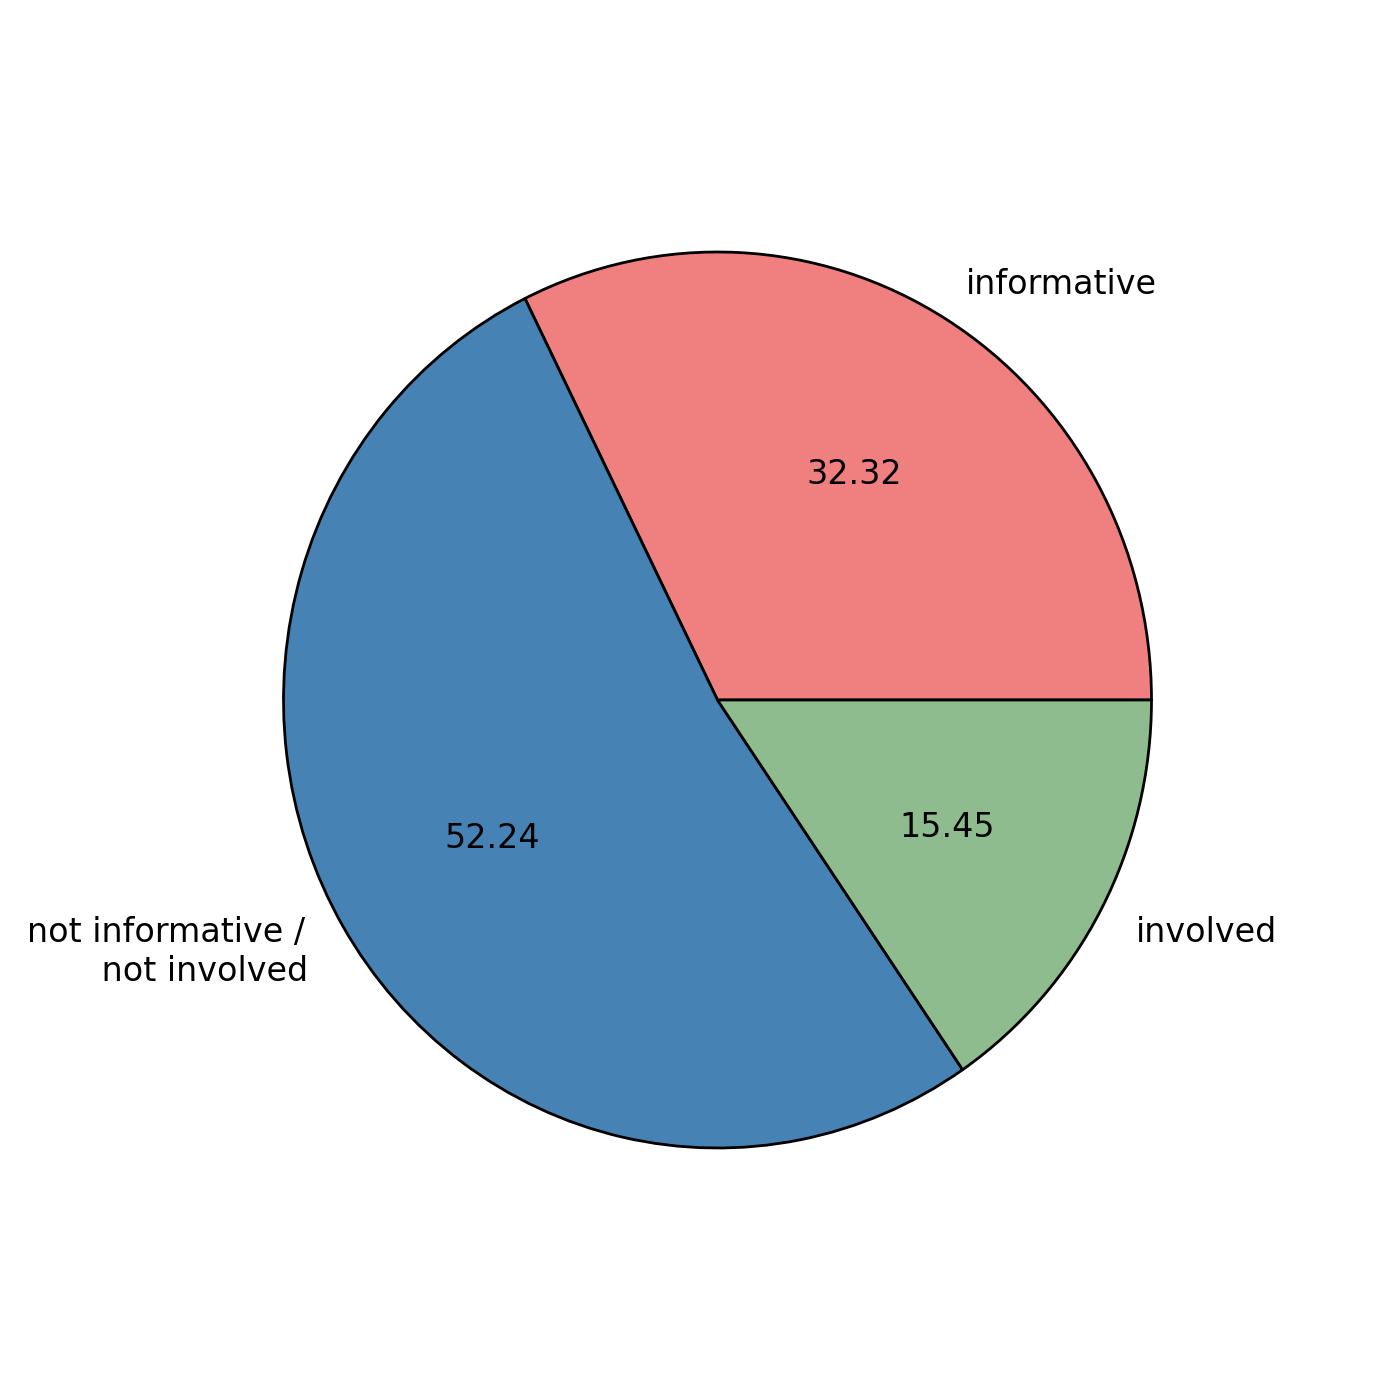
\includegraphics[width=0.5\textwidth]{images/plots/pies/pie_pairs3.png}
\caption{Proportions in dataset}
\end{figure}

\begin{figure}[H]
  \centering
\begin{tabular}{c|c|c|c|c||||c|}
\cline{2-6}
& class \# & 0 & 1 & 2 & \multirow{3}{*}{average}\\ \cline{2-5}
% & proportion & 52\% & 32\% & 15\%  & \\ \cline{2-5}
& meaning & $\neg$ if $\&$ $\neg$ iv & if $\&$ $\neg$ iv & $\neg$ if $\&$ iv  & \\
\hline
\multicolumn{1}{|c|}{\multirow{3}{*}{\rotatebox{90}{NB}}} & unigrams & 76.1\% & 72.8\% & 14.5\% & 64.9\% \\
\multicolumn{1}{|c|}{} & bigrams & 74.3\% & 68.4\% & 4.2\% & 61.1\%   \\
\multicolumn{1}{|c|}{} & trigrams & 72\% & 49.2\% & 0\% & 53.2\% \\
\hline
\hline
\multicolumn{1}{|c|}{\multirow{3}{*}{\rotatebox{90}{PNB}}} & unigrams & 68.6\% & 70.0\% & 18.9\% & 60.8\% \\
\multicolumn{1}{|c|}{} & bigrams & 62.5\% & 64.5\% & 10.1\% & 54.6\%   \\
\multicolumn{1}{|c|}{} & trigrams & 35.4\% & 46.9\% & 0\% & 32.1\% \\
\hline
\end{tabular}
\caption{Accuracies 5-fold cross-validation ; if = informative, iv = involved}
\end{figure}

\newpage

\section{Media analysis}
As seen in the previous part, it is difficult to classifiy the biased tweets only by the language.

\subsection{Motivation}

// almost half of the tweets are medias

// plot of media proportions

If we take a look at the tweets on the 11th of August labeled as biased, we can extract the medias on the figure \ref{tweets500mediasBiaised}. From the left to right column, one can see the domain name of the medias, a description and a manual \emph{dangerousness} classification (1 if dangerous, 0 otherwise).

The medias types are various : videos, images, blog articles, chatting window etc.
\begin{figure}[H]
  \centering
\begin{tabular}{|c|c|c|}
\hline
media domain name & description & class \\ \hline
\texttt{youtube.com} & Anonymous Operation video & 1 \\ \hline
\texttt{cnn.com} & video of Brown's mother "you took my son away from me" & 0 \\
\texttt{vine.co} & a man encouraging the protesters. "No fear. Keep going." & 1 \\ \hline
\texttt{twimg.com} & picture about racism & 0 \\ \hline
\texttt{talk.ee} & chat window & 1 \\ \hline
\texttt{theobamacrat.com} & blog article defending Mike Brown & 0 \\ \hline
\texttt{twitter.com} & tweet/photo of an activist (deleted since) & ? \\ \hline
\texttt{stltoday} & article defending Mike Brown & 0 \\ \hline
\texttt{youtube.com} & video clip encouraging riots & 1 \\ \hline
\hline
\end{tabular}
\label{tweets500mediasBiaised}
\caption{medias in the training sets labelled as involved}
\end{figure}
\newpage
ll
\newpage
\subsection{Formulation}
Let's define $\mathcal{M}_r$ the set of medias $m$ shared during the riot $r$ :
$$ \mathcal{M}_r = \{ m \} $$ 

\subsection{Methods}

\subsubsection{Annoting the top 100 medias}
We first consider the 100 medias the most retweeted on the 11th of the August, and we label it manually :
\begin{itemize}
\item \textbf{garbage} (class 0)
\item \textbf{informative} (class 1)
\item \textbf{biased} (class 2)
\end{itemize}

\begin{figure}[H]
\begin{minipage}[t]{0.45\textwidth}
\begin{center}
	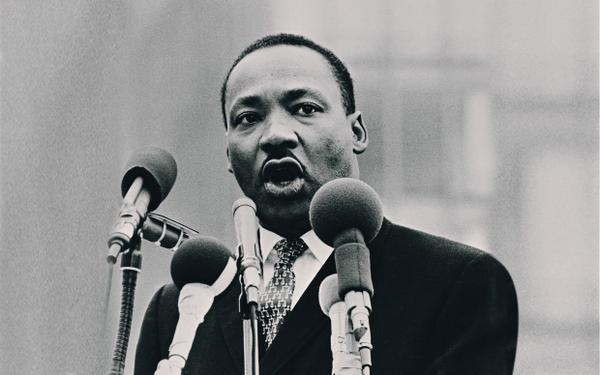
\includegraphics[width=\textwidth]{images/photos/mlk.jpg}
	\caption{Media the most shared on the 11/08 night}
\end{center}
\end{minipage}
\hfill
\begin{minipage}[t]{0.4\textwidth}
\begin{center}
	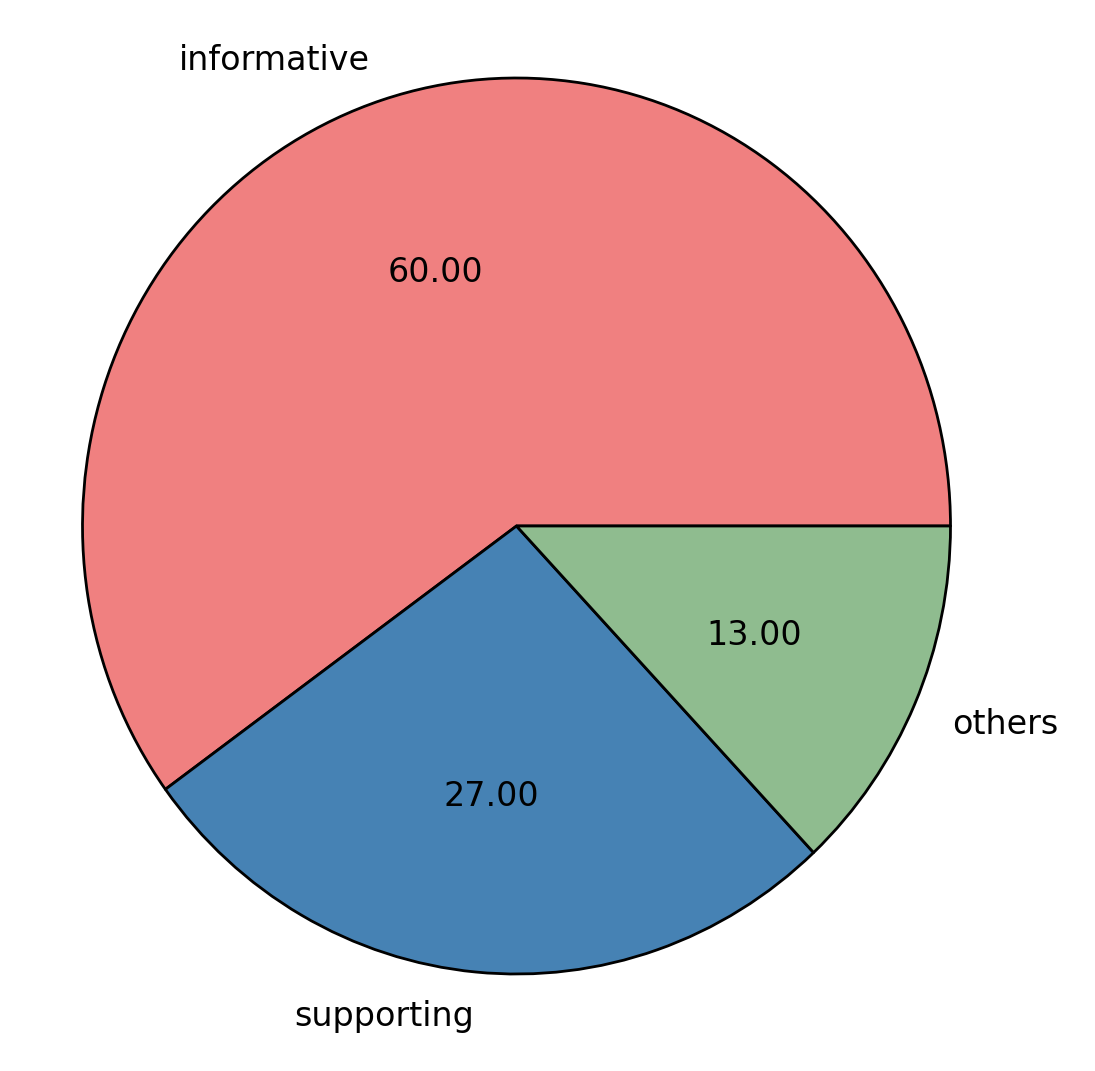
\includegraphics[width=\textwidth]{images/plots/pies/pie_medias.png}
	\caption{Media type repartition on the 11/08}
	\label{typeRepartitionMedias}
\end{center}
\end{minipage}
\end{figure}

The type repartition can be seen on the figure \ref{typeRepartitionMedias}

\newpage

\subsubsection{Media embedding}
Once we have the top 100 medias list, 

\[
\bordermatrix{~ & media_1 & media_2 & \cdots & media_n \cr user_1 =  & tfidf_{1,1} & tfidf_{1,2} & \cdots & tfidf_{1,n} \cr}
\]

\begin{figure}[H]
\centering
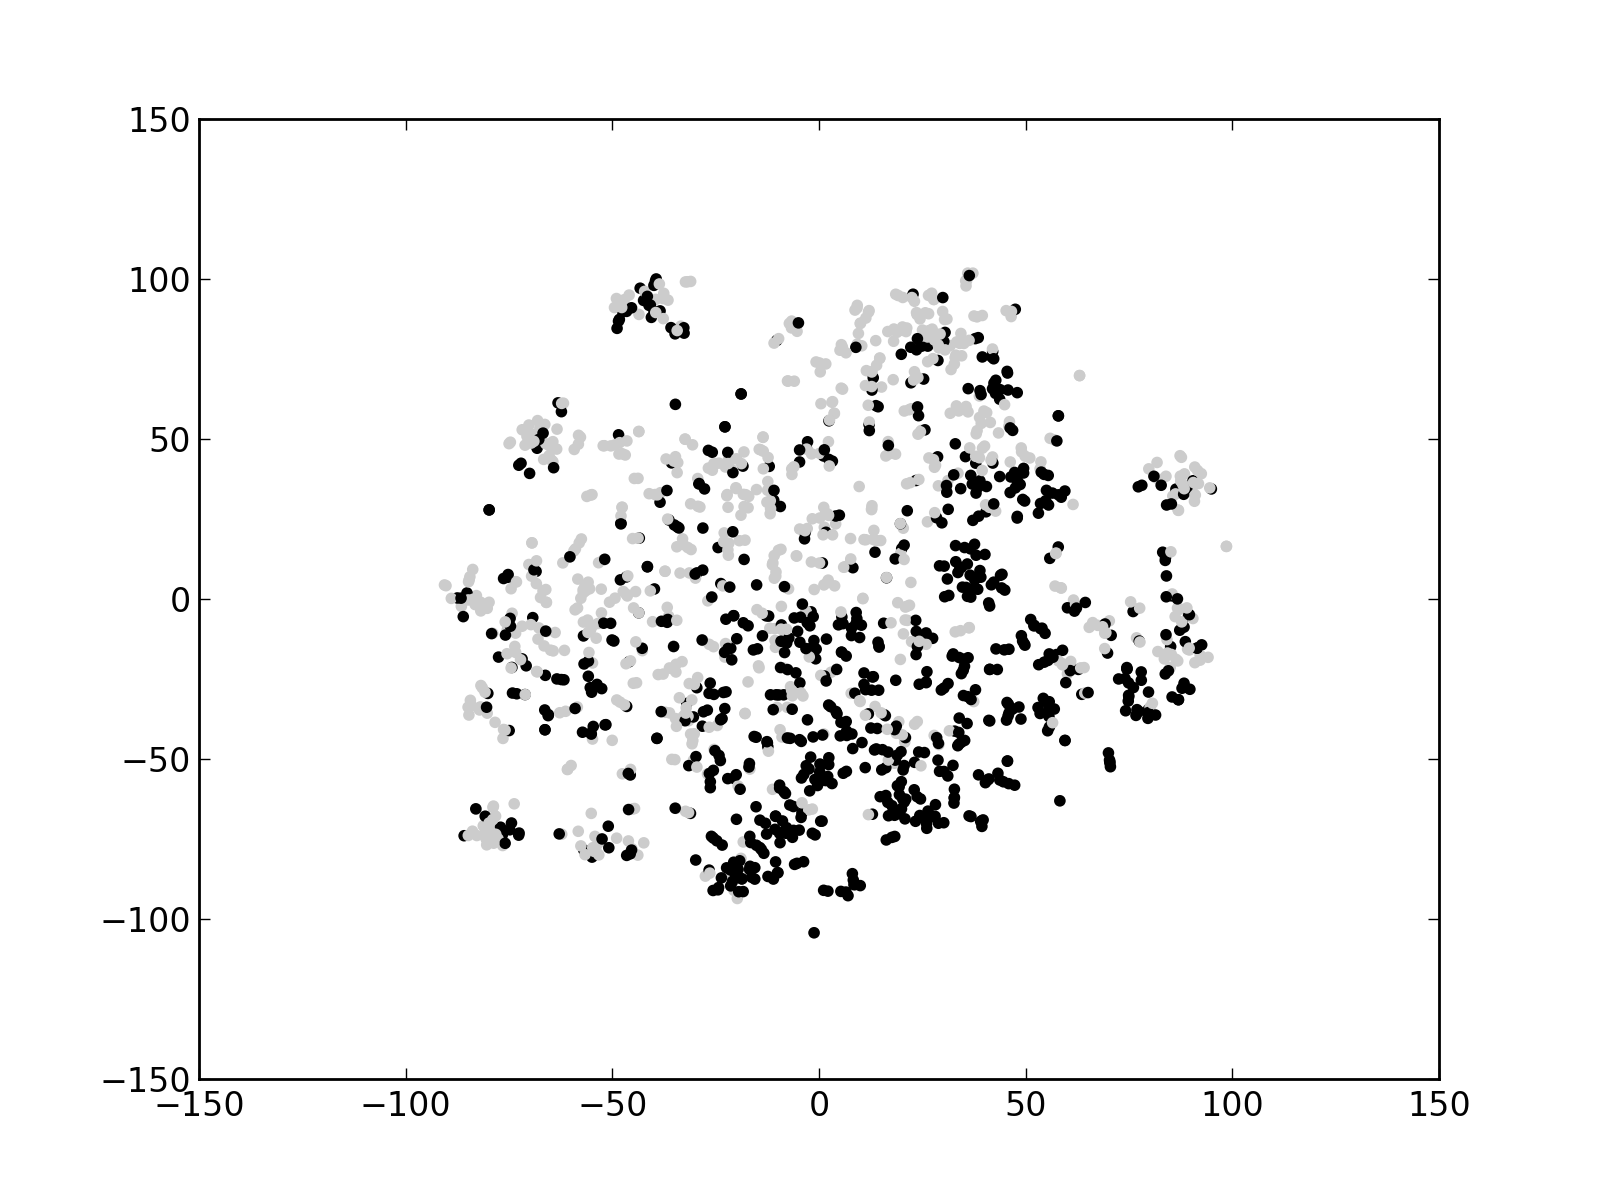
\includegraphics[width=\textwidth]{images/plots/media_tsne.png}
\caption{tsne}
\end{figure}

\begin{figure}[H]
  \centering
\begin{tabular}{c|c|c|c|c||||c|}
\cline{2-6}
& class \# & 0 & 1 & 2 & \multirow{2}{*}{average}\\ \cline{2-5}
& meaning & $\neg$ if $\&$ $\neg$ iv & if $\&$ $\neg$ iv & $\neg$ if $\&$ iv  & \\
\hline
\multicolumn{1}{|c|}{\multirow{3}{*}{\rotatebox{90}{NB}} } & unigrams & 68.4\% & 93.2\% & 81.2\% & 87.1\% \\
\multicolumn{1}{|c|}{} & bigrams & 60.0\% & 90.1\% & 81.2\% & 84.0\%   \\
\multicolumn{1}{|c|}{} & trigrams & 52.2\% & 89.3\% & 81.7\% & 81.8\% \\
\hline
\hline
\multicolumn{1}{|c|}{\multirow{3}{*}{\rotatebox{90}{PNB}}} & unigrams & 67.6\% & 93.1\% & 80.1\% & 86.8\%   \\
\multicolumn{1}{|c|}{} & bigrams & 60.6\% & 90.1\% & 81.3\% & 84.1\%   \\
\multicolumn{1}{|c|}{} & trigrams & 52.1\% & 89.6\% & 81.6\% & 81.8\% \\
\hline
\end{tabular}
\caption{Accuracies 5-fold cross-validation ; if = informative, iv = involved}
\end{figure}

%%%%%%%%%%%%%%%%%%%%%%%%%%%%%%%%%%%%%%%%%%%%%%%%%%%%%%%%%%%%%%%%%%%%%%%
%%%%%%%%%%%%%%%%%%%%%%%%%%%%%%%%%%%%%%%%%%%%%%%%%%%%%%%%%%%%%%%%%%%%%%%
%%%%%% CHAPTER 4 - DETECTING TOPICS
%%%%%%%%%%%%%%%%%%%%%%%%%%%%%%%%%%%%%%%%%%%%%%%%%%%%%%%%%%%%%%%%%%%%%%%
%%%%%%%%%%%%%%%%%%%%%%%%%%%%%%%%%%%%%%%%%%%%%%%%%%%%%%%%%%%%%%%%%%%%%%%

\chapter{Tweets clustering : detecting topics}

\section{Motivation}
The other question one may wonder is what the tweets are talking about, what are the main topics discussed during the riot. \\

On one hand, considering only the informative tweets, the topic detection can tell what is happening, which is the facts and breaking news concerning a riot.
\newpage

\section{Tweet embedding}

The goal is to characterize a tweet by the words it contains, by using for example the bag-of-words representation.

However, this method has its limits. Indeed, it does not consider how a word is common or not inside the whole corpus of tweets. For example, the word "Ferguson" is not very useful to characterize a tweet as it is a very common word in the corpus.

Instead, it is preferable to compute the TF-IDF, for term frequency – inverse document frequency, particularly used in text mining.

It is defined as follow : 

$$tfidf = tf \times idf$$ 
where 
$tf$ is the frequency of the word in the considered document (tweet) and
$$idf = log \frac{|D|}{|\{d_j | t_j \in d_j\}|}$$
where $D = \{d_j | j\in R\} $ is the set of documents (tweets) and $|.|$ is defined as the size of the set.

In this way, for each word of a tweet, we take into consideration if this word is common in the dataset or not, and ajust its frequency accordingly. This method allows to bring out the uncommon words that may characterize a tweet.

We are now able to represent a tweet in the space of the vocabulary words $\mathcal{V}$ :

\[
\bordermatrix{~ & word_1 & word_2 & \cdots & word_n \cr tweet =  & tfidf_1 & tfidf_2 & \cdots & tfidf_n \cr}
\]

And all the tweets vectors generate the term matrix $\mathcal{M}$ :

\[
\bordermatrix{
~ & word_1 & word_2 & \cdots & word_n \cr 
tweet_1 & tfidf_{1,1} & tfidf_{1,2} & \cdots & tfidf_{1,n} \cr
tweet_2 & tfidf_{2,1} & tfidf_{2,2} & \cdots & tfidf_{2,n} \cr
\vdots & \vdots & \vdots & \ddots & \vdots \cr
tweet_m & tfidf_{m,1} & tfidf_{m,2} & \cdots & tfidf_{m,n} \cr
}
\]

\newpage

\section{Distance between two tweets}

\subsection{Euclidean distance}
In order to evaluate if two tweets are close or not, distance functions.\\
we need a distance function $\mathcal{D}$ such that
$$ \mathcal{D} : X\times X \rightarrow \textbf{\textsf{R}}^+ $$
and such that $\mathcal{D}$, for all $t_1$,$t_2$ $\in X$
\begin{itemize}
\item $\mathcal{D}(t_1,t_2)$ is \textbf{small} if $t_1$ and $t_2$ are \textbf{similar}
\item $\mathcal{D}(t_1,t_2)$ is \textbf{large} if $t_1$ and $t_2$ are \textbf{dissimilar}
\end{itemize}
the most commonly used distance define as follow :
$$ \forall t_1,t_2 \in X, \mathcal{D}(t_1,t_2) = || t_1 - t_2 ||_2 $$


\subsection{Cosine similarity}

we need a similarity function $\cos$ such that
$$ \cos : X\times X \rightarrow \textbf{\textsf{R}}^+ $$
and such that $\cos$, for all $t_1$,$t_2$ $\in X$
\begin{itemize}
\item $\cos(t_1,t_2)$ is \textbf{small} if $t_1$ and $t_2$ are \textbf{dissimilar}
\item $\cos(t_1,t_2)$ is \textbf{large} if $t_1$ and $t_2$ are \textbf{similar}
\end{itemize}

$$ \forall t_1,t_2 \in X, \cos(t_1,t_2) = \frac{t_1.t_2}{||t_1||.||t_2||} $$

\newpage
\section{Clustering using $k$-means}

\subsection{$k$-means algorithm}
Given a set of documents $\mathcal{C} = \{d_1,d_2,\cdots,d_m\}$, we want to find $k$ centers, or topics, $t_1,t_2,\cdots,t_k$ that minimizes the cost :
$$ \sum_{i=1}^n \min_j ||d_i-t_j||_2^2 $$


\begin{algorithm}
\caption{$k$-means algorithm}
\label{algo:kmeans}
\begin{algorithmic} 
\STATE pick randomly $k$ center ${t_1,t_2,\cdots,t_k}$
\REPEAT
\STATE assign each point $d$ to its closest center t, in order to create $k$ clusters
\STATE compute the new centers by taking the mean of each cluster
\UNTIL{convergence}
\end{algorithmic}
\end{algorithm}

For a better initialization, some improved algorithms like $k$-means++ exist.


\subsection{Experiment}

\subsection{Limits}

\newpage
\section{Latent Dirichlet Allocation}

\subsection{LDA algorithm}

\begin{center}
\begin{tabular}{ll}
Topics & $ \mathcal{T} = \{t_1,t_2,\cdots,t_k\} $ \\
Documents & $ \mathcal{C} = \{d_1,d_2,\cdots,d_m\} $ \\
Vocabulary & $ \mathcal{V} = \{w_1,w_2,\cdots,w_n\} $ \\
\end{tabular}
\end{center}

Let's consider that : 
\begin{enumerate}
\item each document is a probabilistic mixture of several underlying topics ;
\item each topic is a probabilistic distribution of words ;
\end{enumerate}

The topics are latent, hidden, as we do not observe them directly. They have to be infered from the words they are described with.

\subsubsection{Dirichlet distribution}
For three topics, the Dirichlet distribution for a document can be visualize in a triangle, as on figure \ref{diri_distri1}. Each corner represent a topic. The closer a document is to a corner, the higher is the probability that the document belongs to the topic. For example, on the figure \ref{diri_distri1}, the document belongs to the topic 2 with an higher probability than with the topics 1 and 3.

\begin{figure}[H]
\begin{minipage}[t]{0.48\textwidth}
\begin{center}
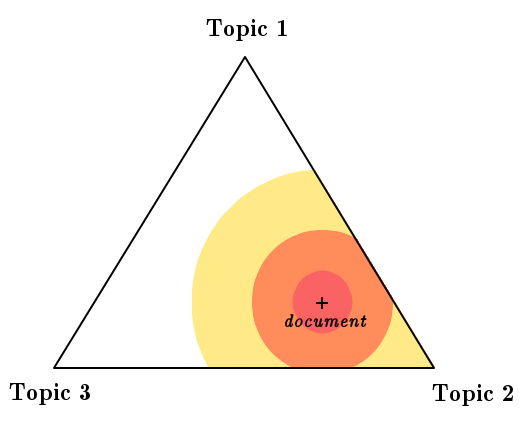
\includegraphics[width=\textwidth]{images/diags/lda_1.png}
\caption{Hashtag graph}
\label{diri_distri1}
\end{center}
\end{minipage}
\hfill
\begin{minipage}[t]{0.48\textwidth}
\begin{center}
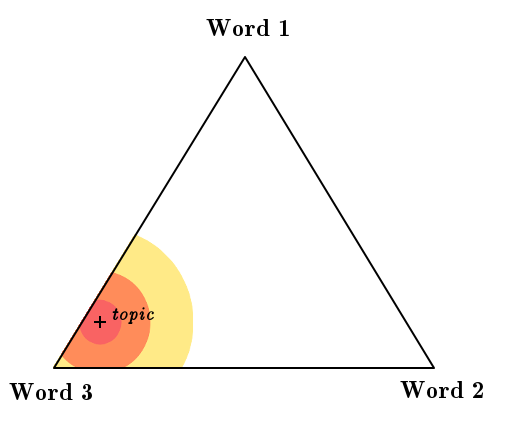
\includegraphics[width=\textwidth]{images/diags/lda_2.png}
\caption{Hashtag graph}
\label{diri_distri2}
\end{center}
\end{minipage}
\end{figure}

As figure \ref{diri_distri2} shows, we also have a Dirichlet distribution for the a topic and words (here 3 words). In this simple example, the topic is mostly characterized by the word 3, and a bit more by the word 1 than the word 2.

distribution of the topics $\beta$\\
topic proportions $\theta$\\

LDA follows the generate process : 
\begin{algorithm}
\caption{LDA : Generative process}
\label{algo:hashtagsGraph}
\begin{algorithmic} 
\FOR{each document $d$}
\STATE draw a distribution over topics $\theta_d \sim \textsf{Dirichlet}(\alpha)$
\FOR{each word $i$ in the document}
\STATE draw a topic $t$ in $\{t_1,\cdots,t_k\}$ according to $\theta_d$
\STATE draw the observed word $w$ according to $\beta_t$
\ENDFOR
\ENDFOR
\\[10pt]
\end{algorithmic}
\end{algorithm}

\subsubsection{Learning process}
The learning process consists of getting topics distributions and proportions according to the considered documents in the corpus.\\

// online learning algorithm 


\newpage

\subsection{Experiment}

\begin{figure}[H]
  \centering
\begin{tabular}{l}
\hline
racial profiling come shoot youth usa dont lessons survival black \\ \hline
right prayers language king unheard luther riot jr martin qt \\ \hline
praying officer police taco bell people swat news team pray \\ \hline
riots quiktrip today august watts ago began years burning tonight \\ \hline
quicktrip ground happening burning police looting gas tear wow scanner \\ \hline
photo burning quicktrip dogs community becomes police blame attention people \\ \hline
purge looting death mo people see guard via right police \\ \hline
police whats going nothing dellwood crazy difference changed pictures color \\ \hline
brown chaos looted police mike killed want looting shop oh \\ \hline
fired shots walmart live video fire police florissant looting quicktrip \\ \hline
\end{tabular}
\caption{Topics obtained by LDA on the 11/08}
\end{figure}

\newpage


%%%%%%%%%%%%%%%%%%%%%%%%%%%%%%%%%%%%%%%%%%%%%%%%%%%%%%%%%%%%%%%%%%%%%%%
%%%%%%%%%%%%%%%%%%%%%%%%%%%%%%%%%%%%%%%%%%%%%%%%%%%%%%%%%%%%%%%%%%%%%%%
%%%%%% CHAPTER 5 - INFLUENCE NETWORK
%%%%%%%%%%%%%%%%%%%%%%%%%%%%%%%%%%%%%%%%%%%%%%%%%%%%%%%%%%%%%%%%%%%%%%%
%%%%%%%%%%%%%%%%%%%%%%%%%%%%%%%%%%%%%%%%%%%%%%%%%%%%%%%%%%%%%%%%%%%%%%%

\chapter{Graph analysis and influence network}

\section{Motivation}

\newpage
\section{Tweets graph}
Considering Twitter features, the most straightforward approach is to study the hashtags. The algorithm \ref{algo:hashtagsGraph} builds a graph of the hashtags combinaisons.

\begin{algorithm}
\caption{Create hashtags graph}
\label{algo:hashtagsGraph}
\begin{algorithmic} 
\STATE \textbf{input} : tweets list, empty graph
\STATE \textbf{output} : graph
\FOR{each tweet in list}
\FOR{each hashtag}
	\STATE add hashtag to list
	\IF{node 'hashtag' does not exist in graph}
	\STATE add hashtag node to graph
	\ENDIF
	\FOR{each couple in 2-permutations of list elements}
	\IF{edge 'couple' does not exist in graph}
	\STATE add couple edge to graph
	\ELSE
	\STATE increase weight of the couple edge in graph
	\ENDIF
	\ENDFOR
\ENDFOR   
\ENDFOR
\\[10pt]
\hspace{-22pt}
\greybox{$\rhd$ \textbf{\underline{Complexity}}: 
The number of hashtags in a tweet is low (en general below 5 and often 0). Thus, for the time complexity we only consider the first for loop, which gives us a \textbf{$\mathcal{O}(n)$} time complexity.
}
\end{algorithmic}
\end{algorithm}

\begin{figure}[H]
\centering
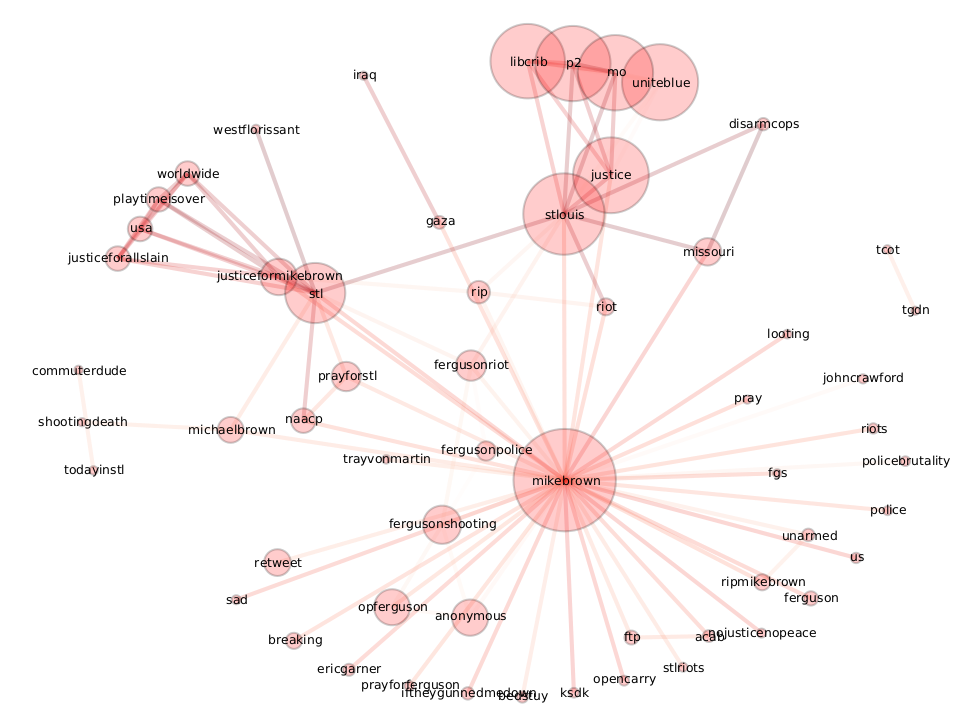
\includegraphics[width=\textwidth]{images/graphs/hashtags/11_08.png}
\caption{Hashtag graph}
\end{figure}

//commentaire communautés
// only the top 100 weighted edges are shown. 

\subsection{Usage}
\begin{figure}[H]
  \centering
\begin{tabular}{|c|c|c|c|}
\hline
argument & description & format & default value \\ \hline
\texttt{time} & time window & hh:mm hh:mm & null \\ \hline
\texttt{rmtags} & remove hashtags & tag1 tag2 ..  & ferguson, mikebrown \\ \hline
\texttt{comms} & search communities & True/False & False \\ \hline
\texttt{nEdges} & number of top edges to keep & number & 500 \\ \hline
\texttt{nComms} & number of top communities to keep & number & 10\\ \hline
\texttt{allnodes} & print all nodes & True/False & False \\ \hline
\texttt{users} & compute users graphs & True/False & False \\ \hline
\hline
\end{tabular}
\caption{top influent users for the 11/08 02:00-09:00}
\end{figure}

\newpage
\section{User's graph}

We can wonder how users actually contribute to these hashtags communities. Do users frequently tweet with hastags of a same community or tweet in several hashtags communities ? For this purpose, we take the 100 users who tweeted the most in a community and we see if they tweeted in others communities. A big red dot represent a community with a given number, a small dot represent a user. A edge, in blue, links a user and a community. The opacity of the edge represents the proportion of the users tweets. The more the edge is dark blue, the more the user contributed to that community. 

\begin{figure}[H]
\centering
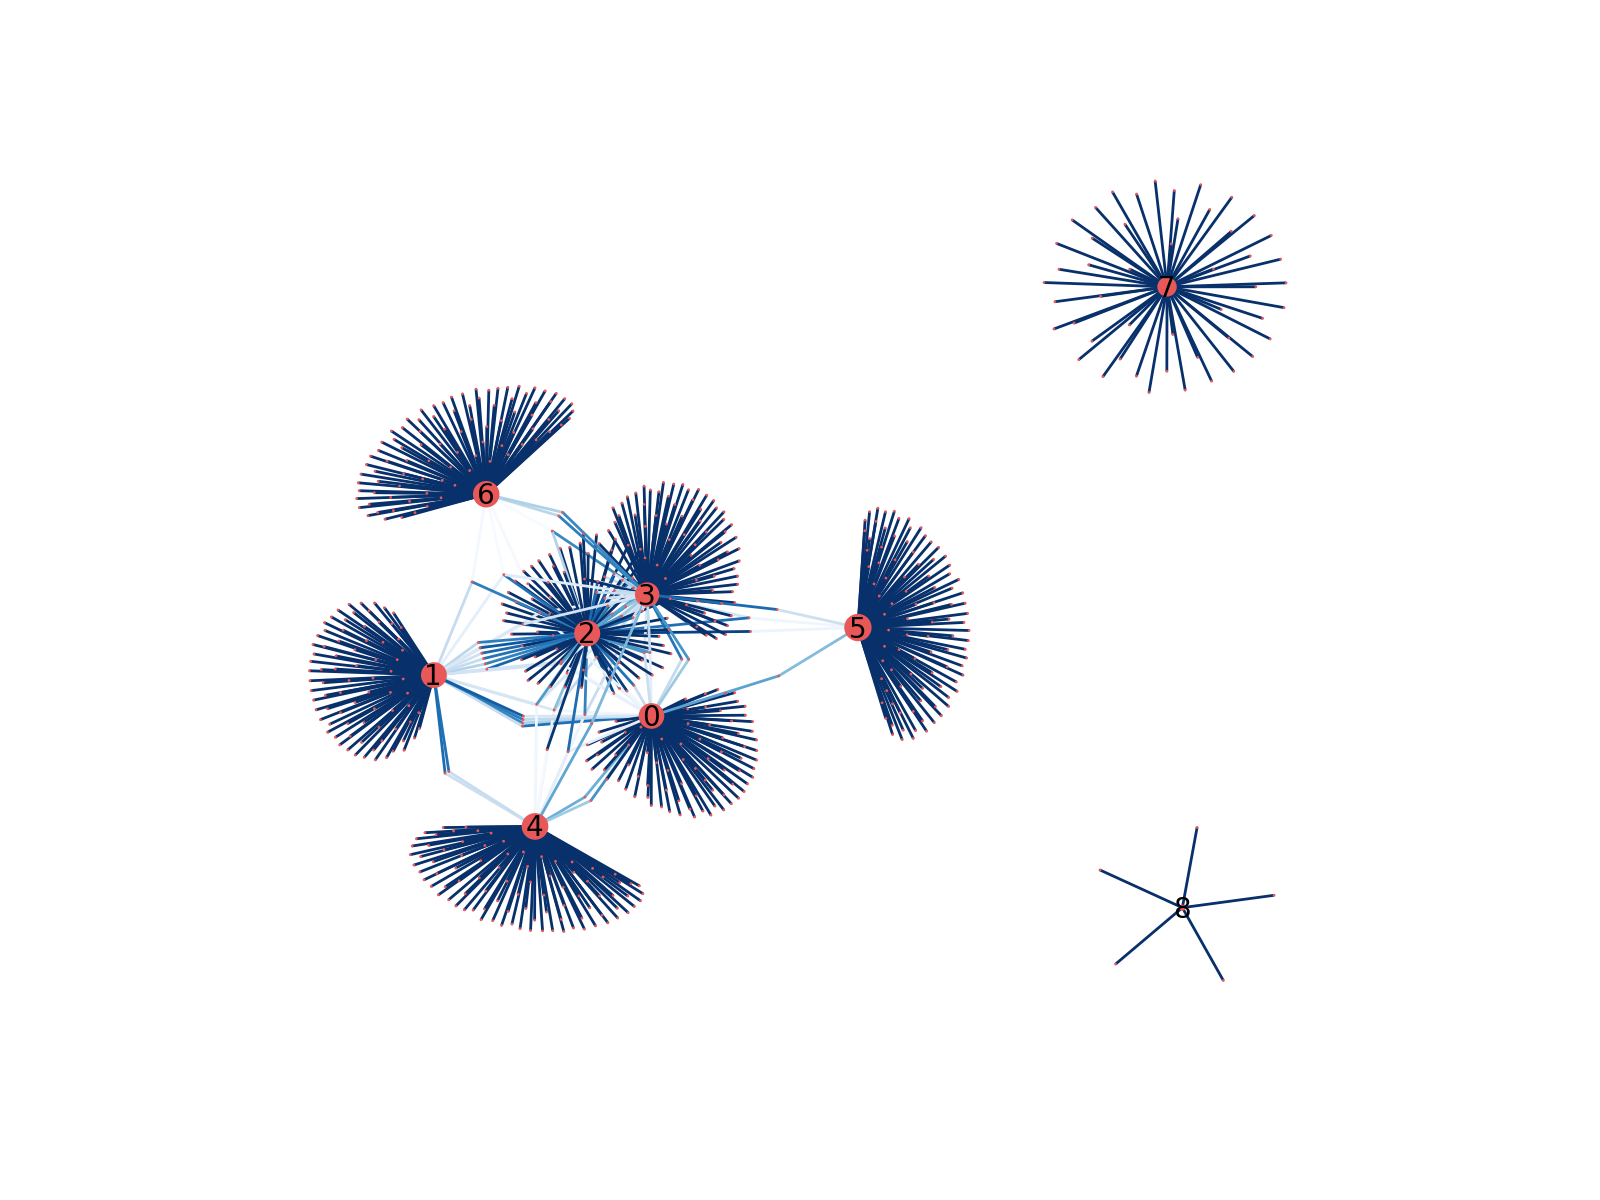
\includegraphics[width=\textwidth]{images/graphs/users/13_08.png}
\caption{Hashtag graph}
\end{figure}

\newpage
\section{Influent users}
\subsection{Centrality and page rank}
\begin{figure}[H]
\centering
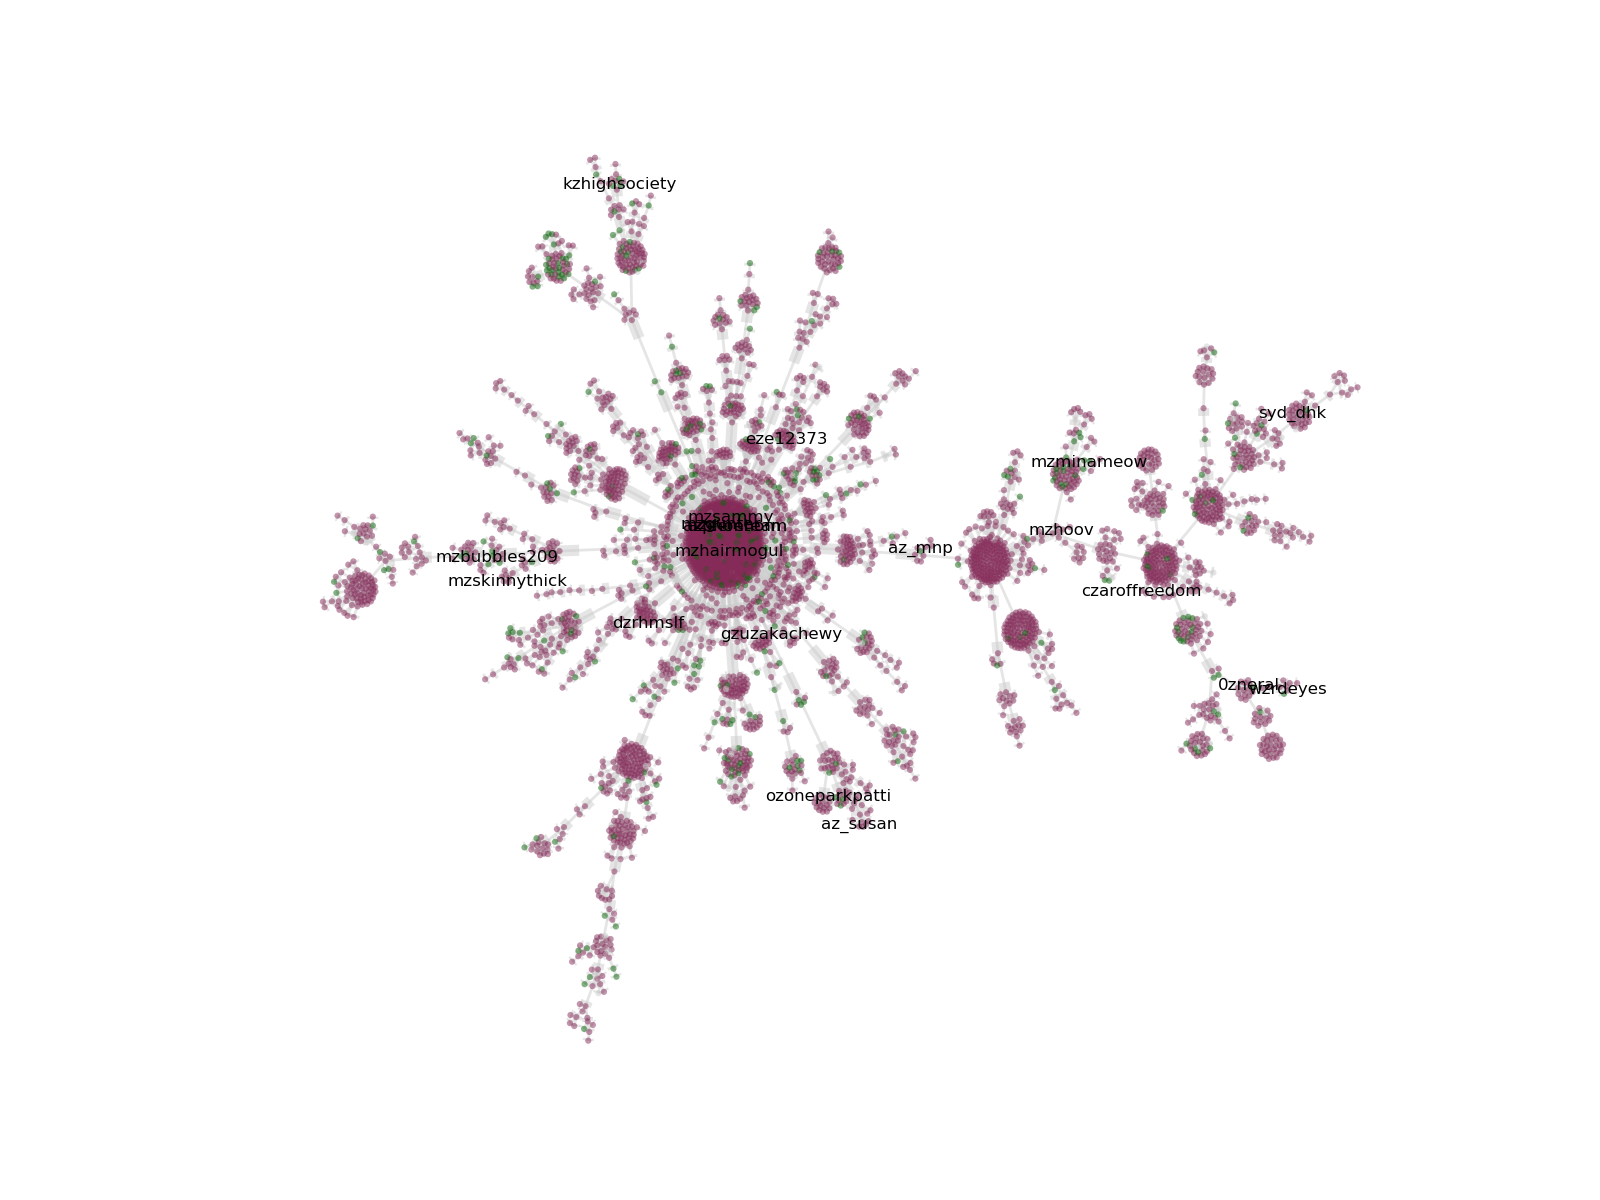
\includegraphics[width=\textwidth]{images/graphs/rtmentions/rtmentions_11_08_02_09.png}
\caption{PageRank}
\end{figure}

\begin{figure}[H]
  \centering
\begin{tabular}{|c|c|c|}
\hline
~ & PageRank & Outdegree Centrality\\ \hline
1 & azeemteam & azeemteam \\ \hline
2 & dzrhmslf & dzrhmslf \\ \hline
3 & 0zneral & 0zneral \\ \hline
4 & mzbubbles209 & mzhairmogul \\ \hline
5 & mzhairmogul & czaroffreedom \\ \hline
6 & czaroffreedom & eze12373 \\ \hline
7 & mzminameow & mzminameow \\ \hline
8 & gzuzakachewy & gzuzakachewy \\ \hline
9 & mzhoov & azphoenom \\ \hline
10 & kzhighsociety & mzhoov \\ \hline
11 & mzskinnythick & kzhighsociety \\ \hline
12 & az\_mnp & mzskinnythick \\ \hline
13 & mzgunter & az\_susan \\ \hline
14 & ozoneparkpatti & mzgunter \\ \hline
15 & wzrdeyes & az\_mnp \\ \hline
16 & eze12373 & ozoneparkpatti \\ \hline
17 & az\_susan & mzbubbles209 \\ \hline
18 & azphoenom & mzsammy \\ \hline
19 & mzsammy & wzrdeyes \\ \hline
20 & syd\_dhk & syd\_dhk\\ \hline
\hline
\end{tabular}
\caption{top influent users for the 11/08 02:00-09:00}
\end{figure}
\subsection{Redefining influence}
\begin{itemize}
\item nombre de tweets différents retweetés par d'autre utilisateurs ;
\item nombre de retweets pour chacun de ces tweets ;
\item si c'est ponctuel ou récurrent
\end{itemize}

\section{Identifying potential dangerous subnetworks}

\chapter{Role of a user}

\section{Definition}
\newpage
\section{Role similarity}
role similarity 1 \newpage
role similarity 2 \newpage
\section{Experiments}
experiment 1 \newpage
experiment 2 \newpage

\chapter{Related work (5p)}
related work 1 \newpage
related work 2 \newpage
related work 3 \newpage

\chapter{Discussion (5p) }
discussion 1 \newpage
discussion 2 \newpage
discussion 3 \newpage

\end{document}
